\chapter{Run-3における近接2ミューオンのためのトリガーアルゴリズムの動作検証}\label{chapter4}

\section{近接2ミューオントリガーアルゴリズム}\label{chapter4-1}
2つのミューオン同士が近接している事象を対象としたバレル領域のミューオントリガーは、近接2ミューオン事象に特化した~L1トリガーと~HLTを組み合わせて用いている。
図~\ref{fig:4-1}にL1とHLTでの2ミューオンの飛跡再構成の流れを示す。

\begin{figure}[H]
    \centering
    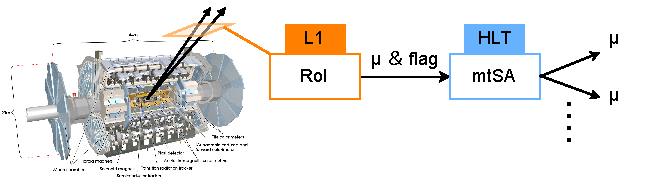
\includegraphics[clip, width=13cm]{fig/4/closebyMuonFlow.pdf}
    \caption{近接2ミューオンのための~L1と~HLTのトリガーを用いたときのデータの流れ。HLTでは複数のミューオンが再構成される。}
    \label{fig:4-1}
\end{figure}

第3章で述べた通りバレル領域の~L1トリガーでは、$\eta-\rm{CM}$と$\phi-\rm{CM}$のコインシデンスを取ることでミューオンの通過位置~RoIを定義するので、1Padあたり1つの~RoIしか出力できない。
そのため近接2ミューオンが同じ~Padを通過した場合でも1つのミューオンとして判定されてしまう。
そこで、2つミューオンが同じ~Padに入ってしまうような近接2ミューオン事象を~L1で判定できるように、既に~L1~RPCに実装されていた近接2ミューオンかどうか判定できるフラグを用いたL1トリガーを~Run-3から導入した。

また~HLTでは~L1から送られてくるフラグの情報と1つの~RoI情報から複数のロードを定義し、複数のミューオンを再構成する~L2MuonSAアルゴリズムが開発、導入された~\cite{article:taniguchi}。

以下で~L1と~HLTそれぞれのアルゴリズムについて説明する。

%\newpage

\subsection{近接2ミューオンのためのL1トリガーアルゴリズム~(L1~BOMトリガー)}\label{chapter4-1-1}
近接2ミューオンのための~L1トリガーは~「L1~Barrel~Only~Multi-trackトリガー~(L1BOMトリガー」と呼ばれる。
この~L1トリガーは、1ミューオントリガーと近接ミューオンを区別するフラグを組み合わせたトリガーである。

\subsubsection{L1近接ミューオンフラグ}
このフラグは以下の図のような同一~Padの異なる~RoIをミューオンが通過したときに、その事象を区別できるフラグである。

\begin{figure}[H]
  \begin{minipage}[b]{0.5\linewidth}
      \centering
      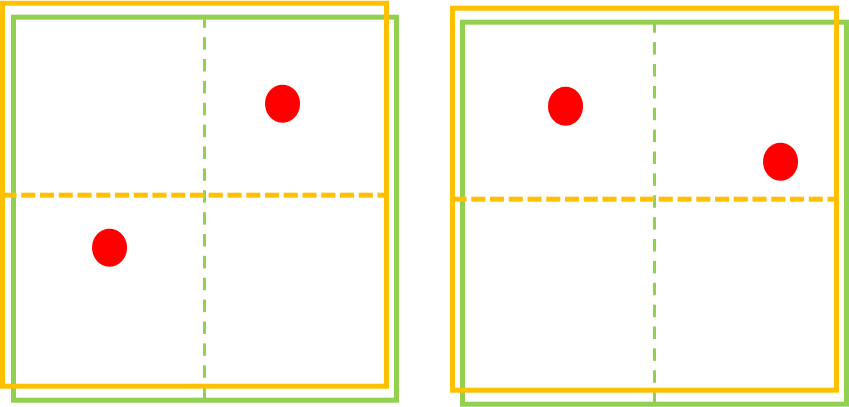
\includegraphics[clip, width=5cm]{fig/4/isflaged.png}
      \subcaption{L1近接2ミューオンフラグが立つ事象}
      \label{fig:4-2-1}
  \end{minipage}
    \begin{minipage}[b]{0.45\linewidth}
      \centering
      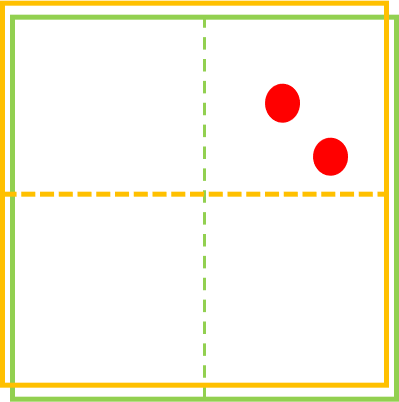
\includegraphics[clip, width=2.5cm]{fig/4/isNotflaged.png}
      \subcaption{L1近接2ミューオンフラグが立たない事象}
      \label{fig:4-2-2}
  \end{minipage}
  \caption{L1近接ミューオンフラグで区別できる2ミューオン事象と区別できない2ミューオン事象。}
\end{figure}

このフラグを用いると、図~\ref{fig:4-2-1}のように同一~Pad内の異なる~RoIを2ミューオンが通過したときに判別することができる。
図~\ref{fig:4-2-2}では$\eta-\rm{CM}$、$\phi-\rm{CM}$ともに1つのみ鳴っているので、単一ミューオン事象と区別がつかずフラグを用いても判別することができない。

\subsection{近接2ミューオンのためのHLTアルゴリズム~(multi-track~SA;mtSA)}\label{chapter4-1-2}
1つの~RoIから複数のミューオンを再構成するための2MuonSAアルゴリズムを「multi-track~Stand~Alone~(mtSA)」と呼ぶ。
mtSAは2つのミューオンが同一~Padを通過するような2ミューオンが非常に近接している事象を対象にしている。

mtSAのアルゴリズムの流れを以下に示す。

\begin{figure}[H]
    \centering
    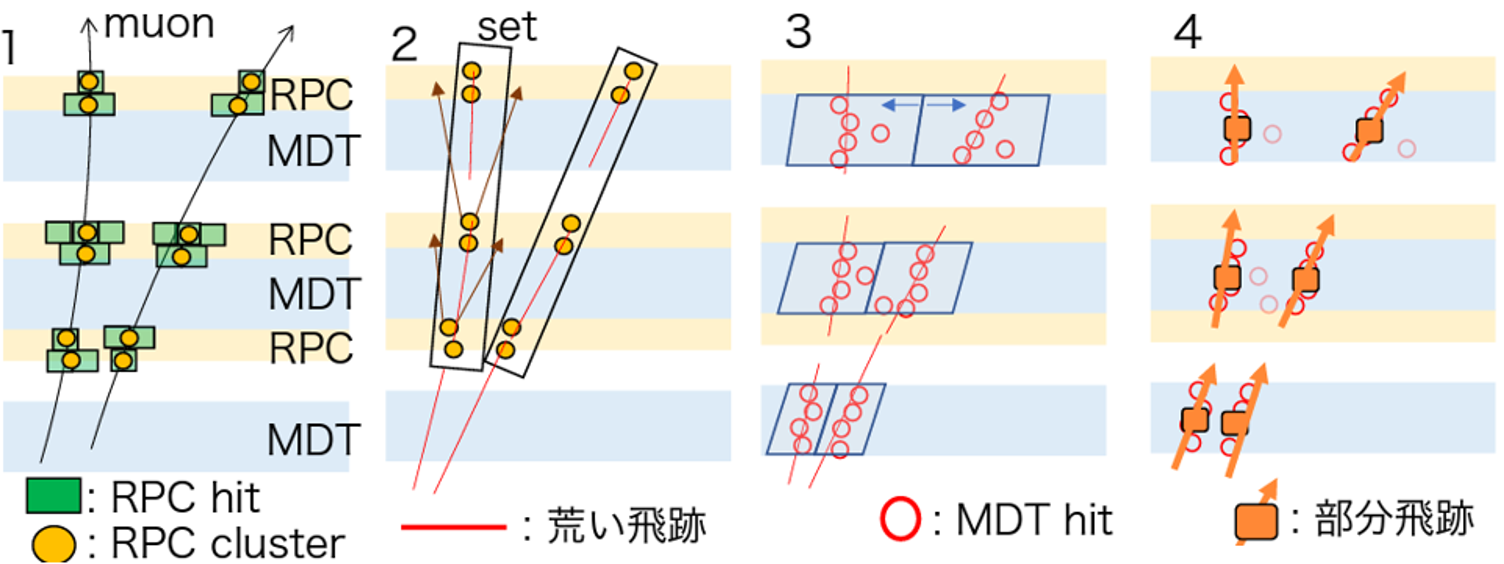
\includegraphics[clip, width=10cm]{fig/4/mtSA_alg.png}
    \caption{mtSAアルゴリズムの流れ\cite{article:taniguchi}}
    \label{fig:4-3}
\end{figure}

\begin{enumerate}
    \item L1から受け取った~RoIの情報を用いてRoI周辺の~RPCのヒット情報を取得し、隣り合う~RPCヒット同士を1つの~clusterとして定義する。このとき各~RPCヒットから~clusterの重心座標を計算し、~clusterの座標とする。
    \item 各層の~RPC~clusterを結ぶ際に、複数の組み合わせを許しロードを定義する。
    \item 2で定義したロードに~MDTのヒットを割り当てる。
    \item 3で割り当てた~MDTヒットから~SPを作成し、$p_{\rm{T}}$を再構成する。
\end{enumerate}

mtSAでは複数のミューオンが同一~Padを通過した事象において、L2MuonSAで複数のミューオンを再構成することを目的する。

\section{トリガー効率の評価方法}\label{chapter4-2}
この節ではトリガー効率の計算方法について述べる。

一般的にトリガー効率を求めるときは、そのトリガーを通過することが期待される事象のうち、実際にトリガーを通過した事象の割合を求める。
ここではトリガーを通過することが期待される事象として、トリガー条件を満たすオフラインで再構成されたミューオンが観測された事象を用いる。
これは2ミューオントリガーの場合も同様で、2ミューオントリガーを通過することが期待される事象のうち、実際に2ミューオントリガーを通過した事象の割合でトリガー効率を評価する。

今回評価した~L1~BOMトリガーはバレル領域に$\SI{10}{\GeV}$以上の$\pt$のミューオン~(RoI)が1つあり、かつフラグが立っていることを要求するので、トリガー効率を以下の式で定義する。

\begin{equation}
    \mathrm{effciency}=\frac{L1~BOMトリガーを通過した事象数}{バレル領域に\pt>\mathrm{\SI{10}{\GeV}}以上のオフラインミューオンが2つある事象数} \label{equ:L1}
\end{equation}

L1~BOMトリガーと既存のL1~2ミューオントリガーのトリガー効率を比較するために、既存の2ミューオントリガーのトリガー効率も同様の式を用いて計算した。

また~mtSAのトリガー効率は、2ミューオン効率の分母となる事象を少ないバイアスで取得している他のトリガーがないため,まず1ミューオン事象を取得しその効率を求め,それに対して2ミューオン事象の効率を求める2段階で評価を行った。
具体的にはまず$\pt$が24GeV以上のミューオンが標準的なトリガーを通過している事象において~mtSAがミューオンを再構成した割合を求めた(mtSAのシングルミューオン検出効率)。
次に$\pt$が10GeV以上のミューオンが2つある事象において~mtSAが1つ以上ミューオンを見つけた事象数に対する~mtSAが2つミューオンを再構成した事象数の割合を求めた(mtSAが2つめのミューオンを検出する効率)。
この2段階で~mtSAが2つ以上ミューオンを再構成するトリガー効率を評価した。

\begin{equation}
    \mathrm{efficiency}=\frac{\mathrm{mtSA}がミューオンを再構成した割合}{\pt>\SI{24}{\GeV}のミューオンが標準的なトリガーを通過している事象数} \label{equ:single}
\end{equation}

\begin{equation}
    \mathrm{efficiency}=\frac{\mathrm{mtSA}が2つミューオンを再構成した事象数}{\pt>\SI{10}{\GeV}のオフラインミューオンが2つかつ\mathrm{mtSA}ミューオンが1つ以上ある事象数}\label{equ:L2mt}
\end{equation}

これらのトリガー効率の評価に、Run-3~(2022-2023)に取得されたデータと$J/\psi \rightarrow \mu\mu$のモンテカルロシミュレーション~(MCシミュレーション)のサンプルを用いた。
実データでは2ミューオンの不変質量が$\SI{2.7}{\GeV}<\mathrm{M}_{\mu\mu}<\SI{3.5}{\GeV}$でそれぞれのミューオンが異なる電荷を持つという条件を要求し、$J \rightarrow \mu\mu$由来のミューオン対を選択した。


\section{Run-3実データを用いた初段トリガーにおける近接2ミューオントリガーの動作検証}\label{chapter4-3}
L1~BOMトリガーのトリガー効率を評価するために用いたサンプルの不変質量$M_{\mu\mu}$と、$\pt$、$\Delta R_{\mu\mu~\mathrm{at~Muon~Spectrometer}}$分布を、実データ、シミュレーションについてそれぞれ図~\ref{fig:L1BOMDataSample}、図~\ref{fig:L1BOMMCSample}に示す。
データの分布は$M_{\mu\mu}$分布には条件をかけていないが、他の分布は~L1~BOMトリガーの効率を求める式~\ref{equ:L1}における分母の条件をかけている。

\begin{figure}[H]
    \begin{tabular}{cc}
      \begin{minipage}[b]{0.48\linewidth}
          \centering
          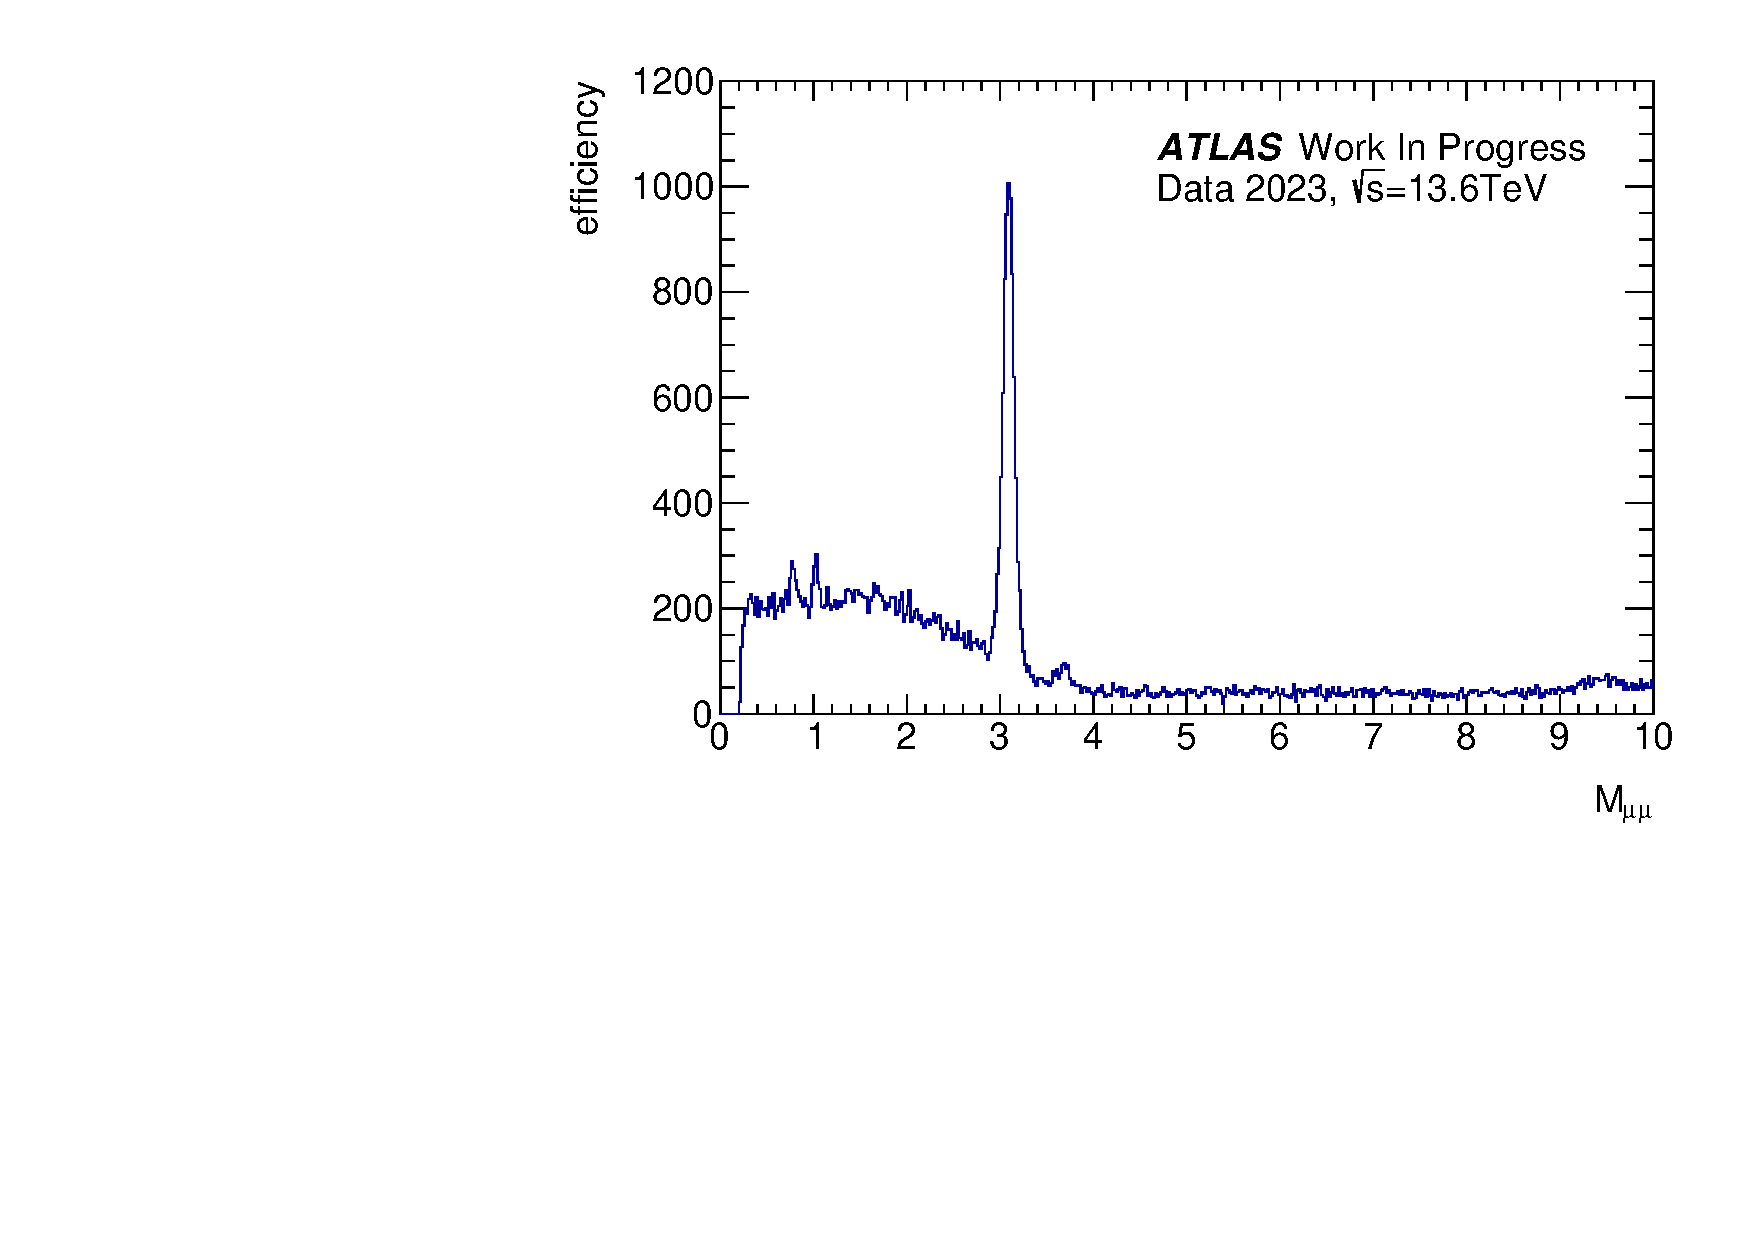
\includegraphics[clip, width=6.5cm]{fig/4/mass_data.pdf}
          \subcaption{$M_{\mu\mu}$分布}
          %\label{fig:5-8-1}
      \end{minipage} &
      \begin{minipage}[b]{0.48\linewidth}
          \centering
          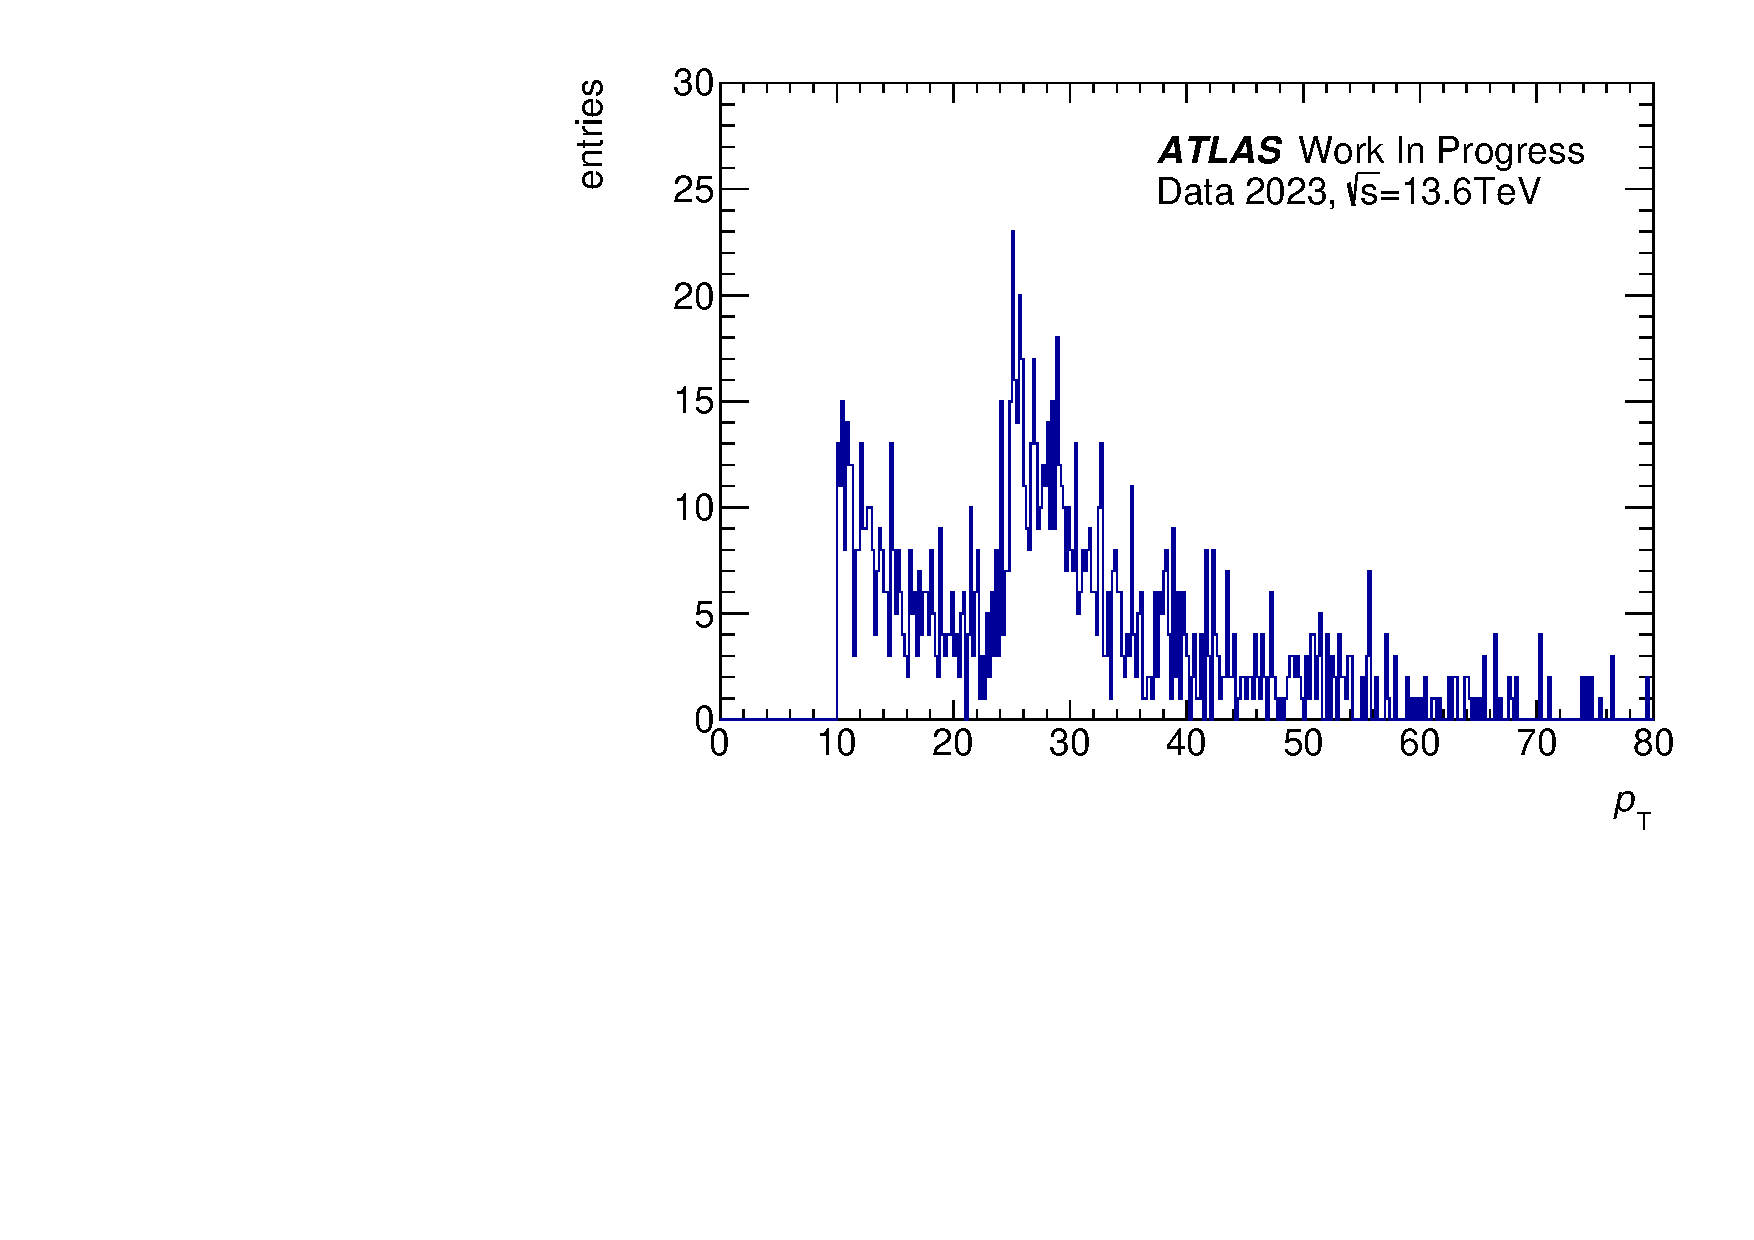
\includegraphics[clip, width=6.5cm]{fig/4/pt_data_v2.pdf}
          \subcaption{$\pt$分布}
          %\label{fig:5-8-2}
      \end{minipage} \\

      \begin{minipage}{0.48\linewidth}
          \centering
          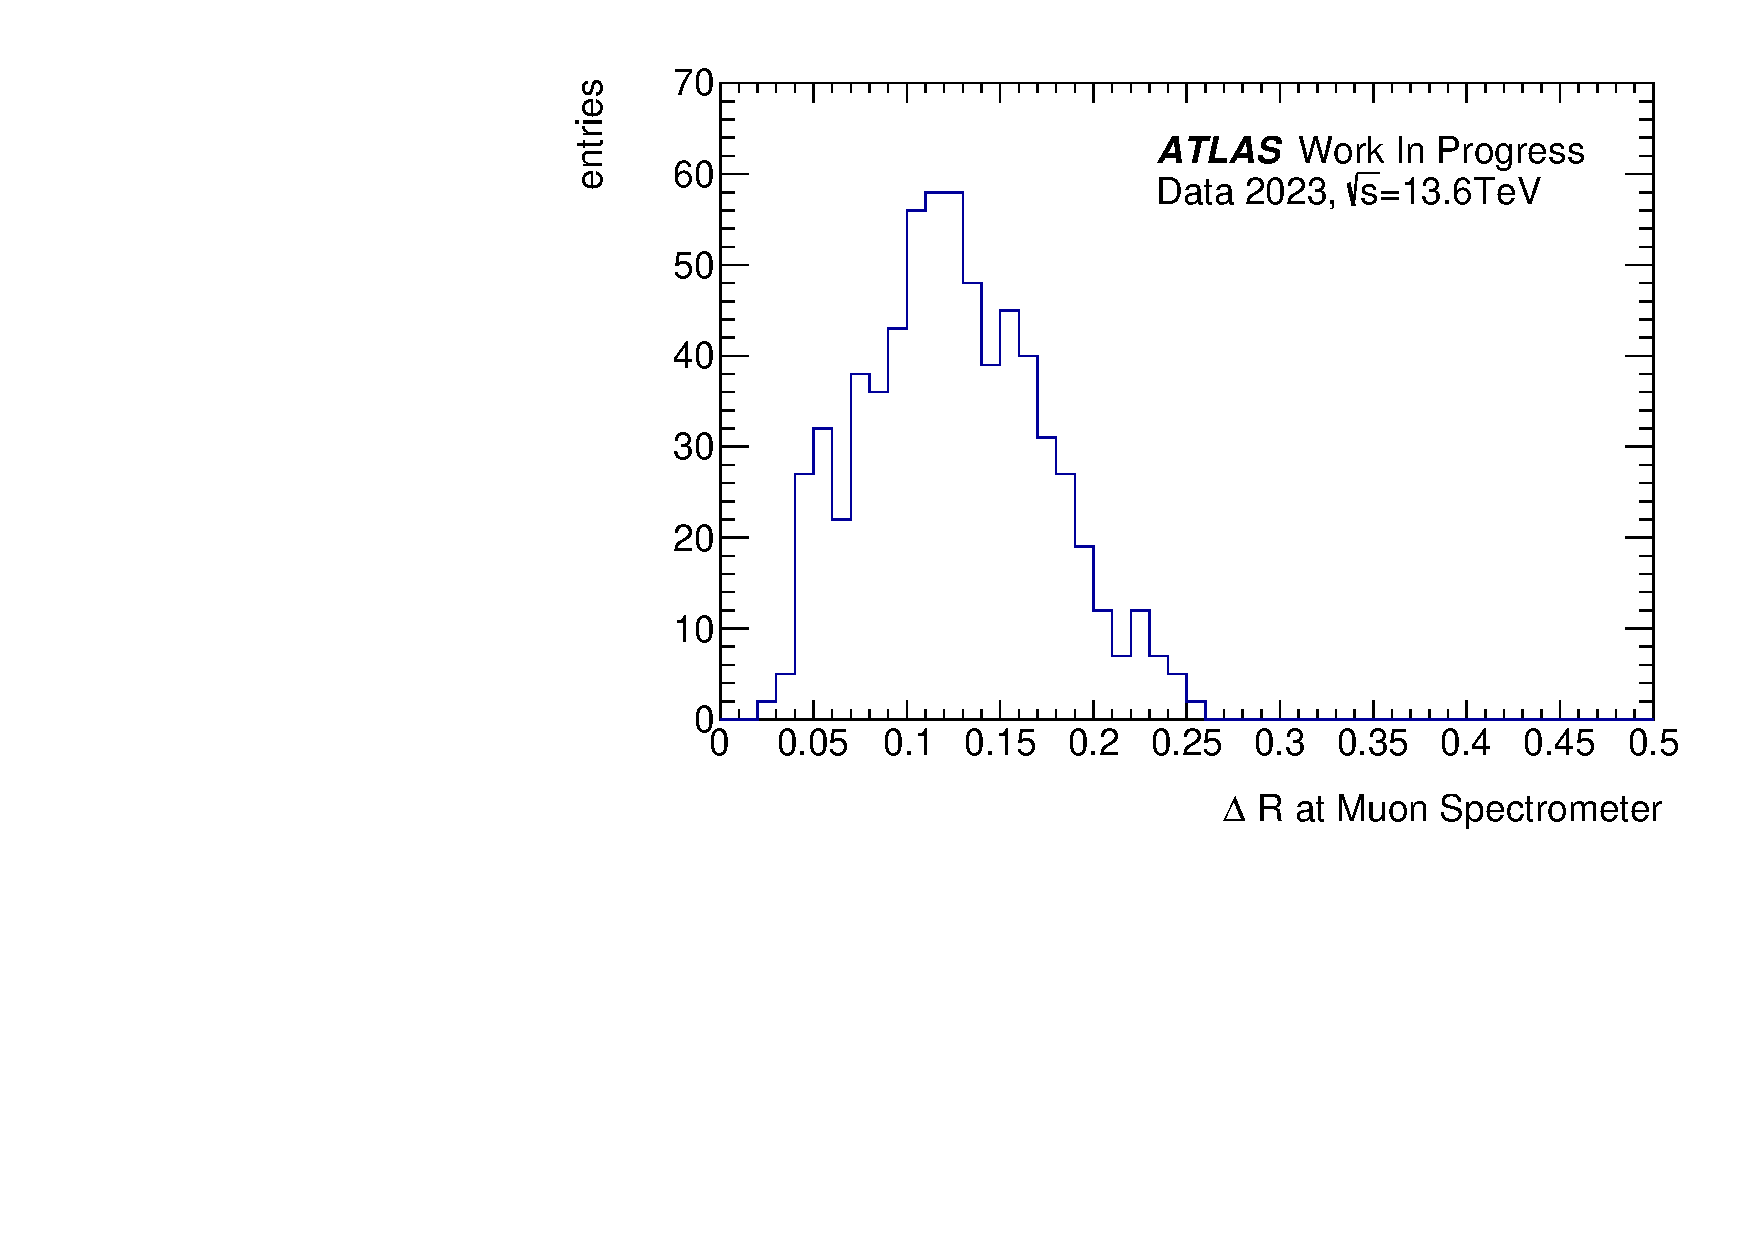
\includegraphics[clip, width=6.5cm]{fig/4/deltaR_ext_data_v2.pdf}
          \subcaption{$\Delta R_{\mu\mu~\mathrm{at~Muon~Spectrometer}}$}
          %\label{fig:5-9-2}
      \end{minipage} \\
    \end{tabular}
    \caption{L1~BOMトリガーのトリガー効率の評価に用いた実データ。}
    \label{fig:L1BOMDataSample}
\end{figure}

\begin{figure}[H]
    \begin{tabular}{cc}
      \begin{minipage}[b]{0.48\linewidth}
          \centering
          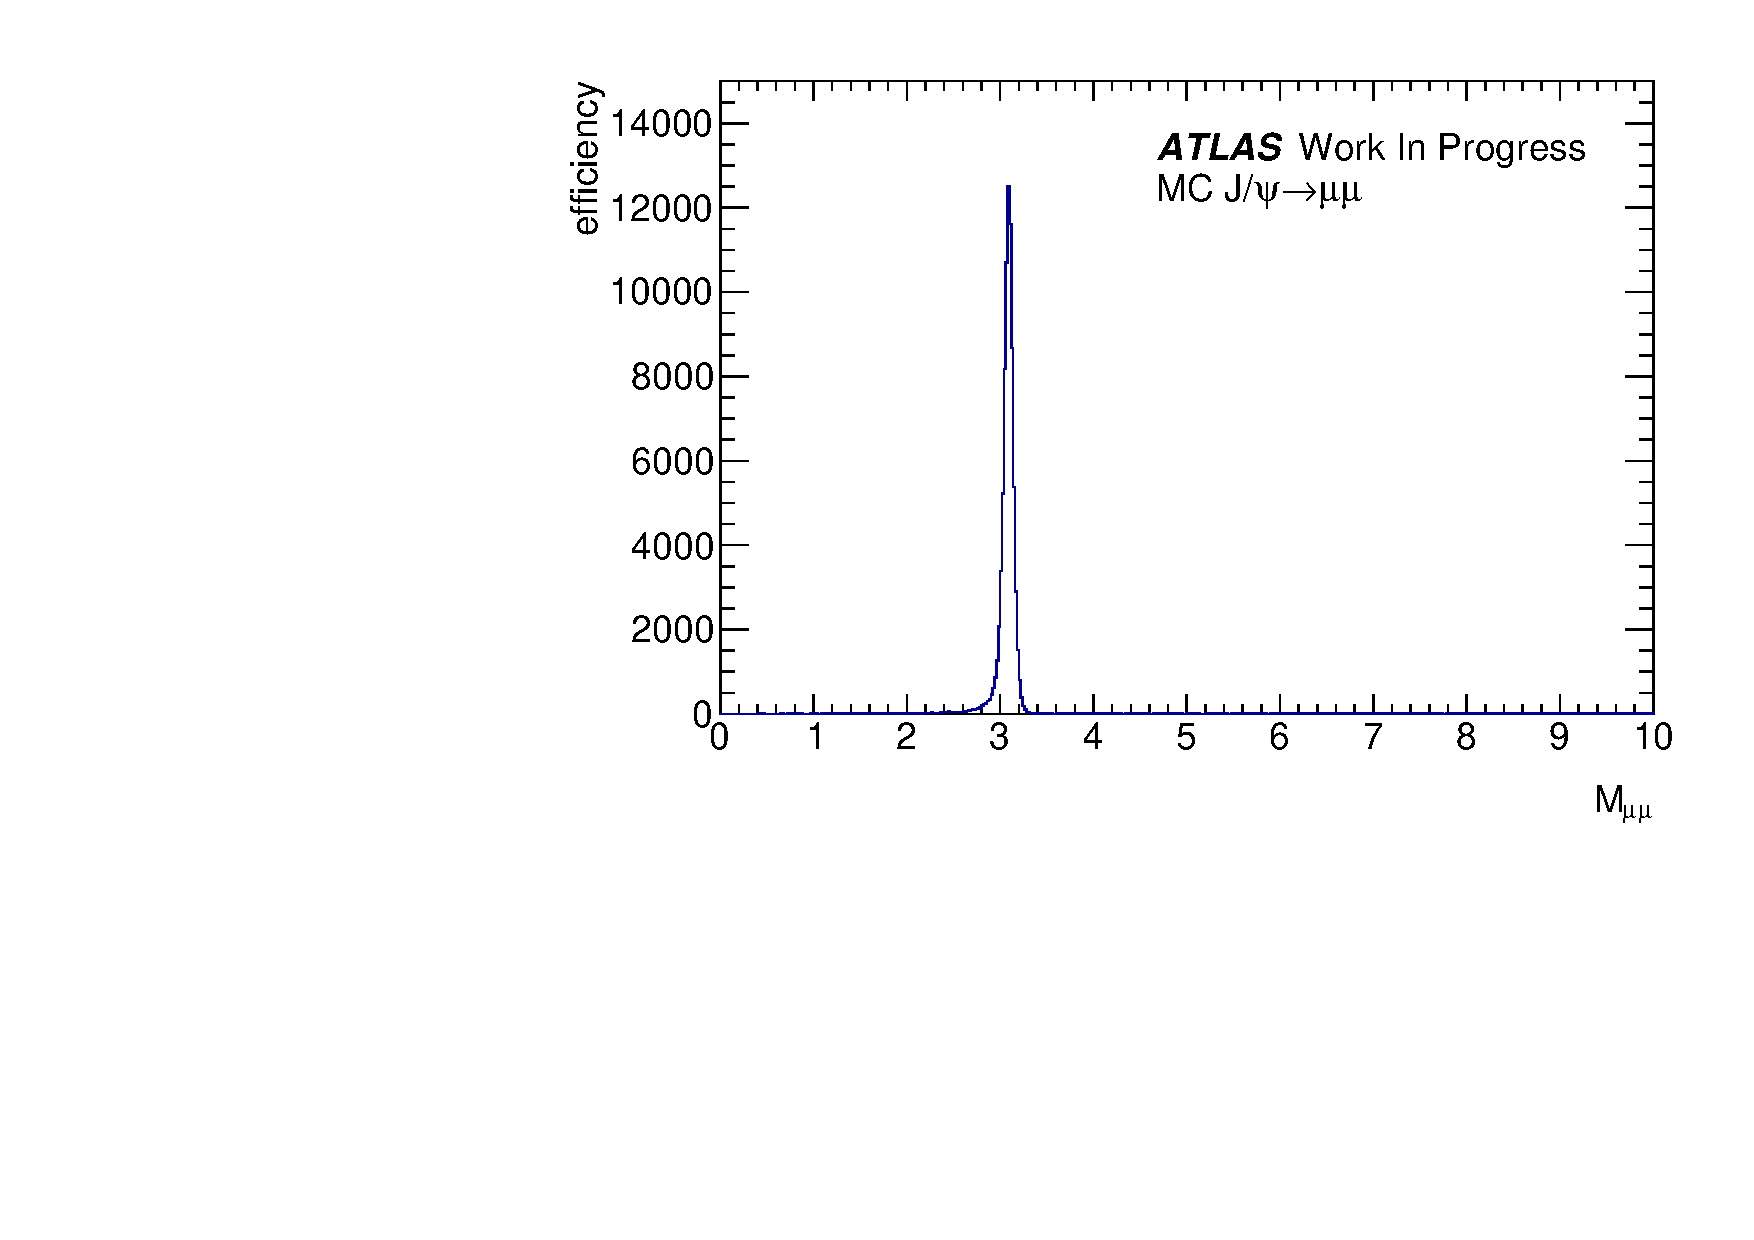
\includegraphics[clip, width=6.8cm]{fig/4/mass_MC.pdf}
          \subcaption{$M_{\mu\mu}$分布}
          %\label{fig:5-8-1}
      \end{minipage} &
      \begin{minipage}[b]{0.48\linewidth}
          \centering
          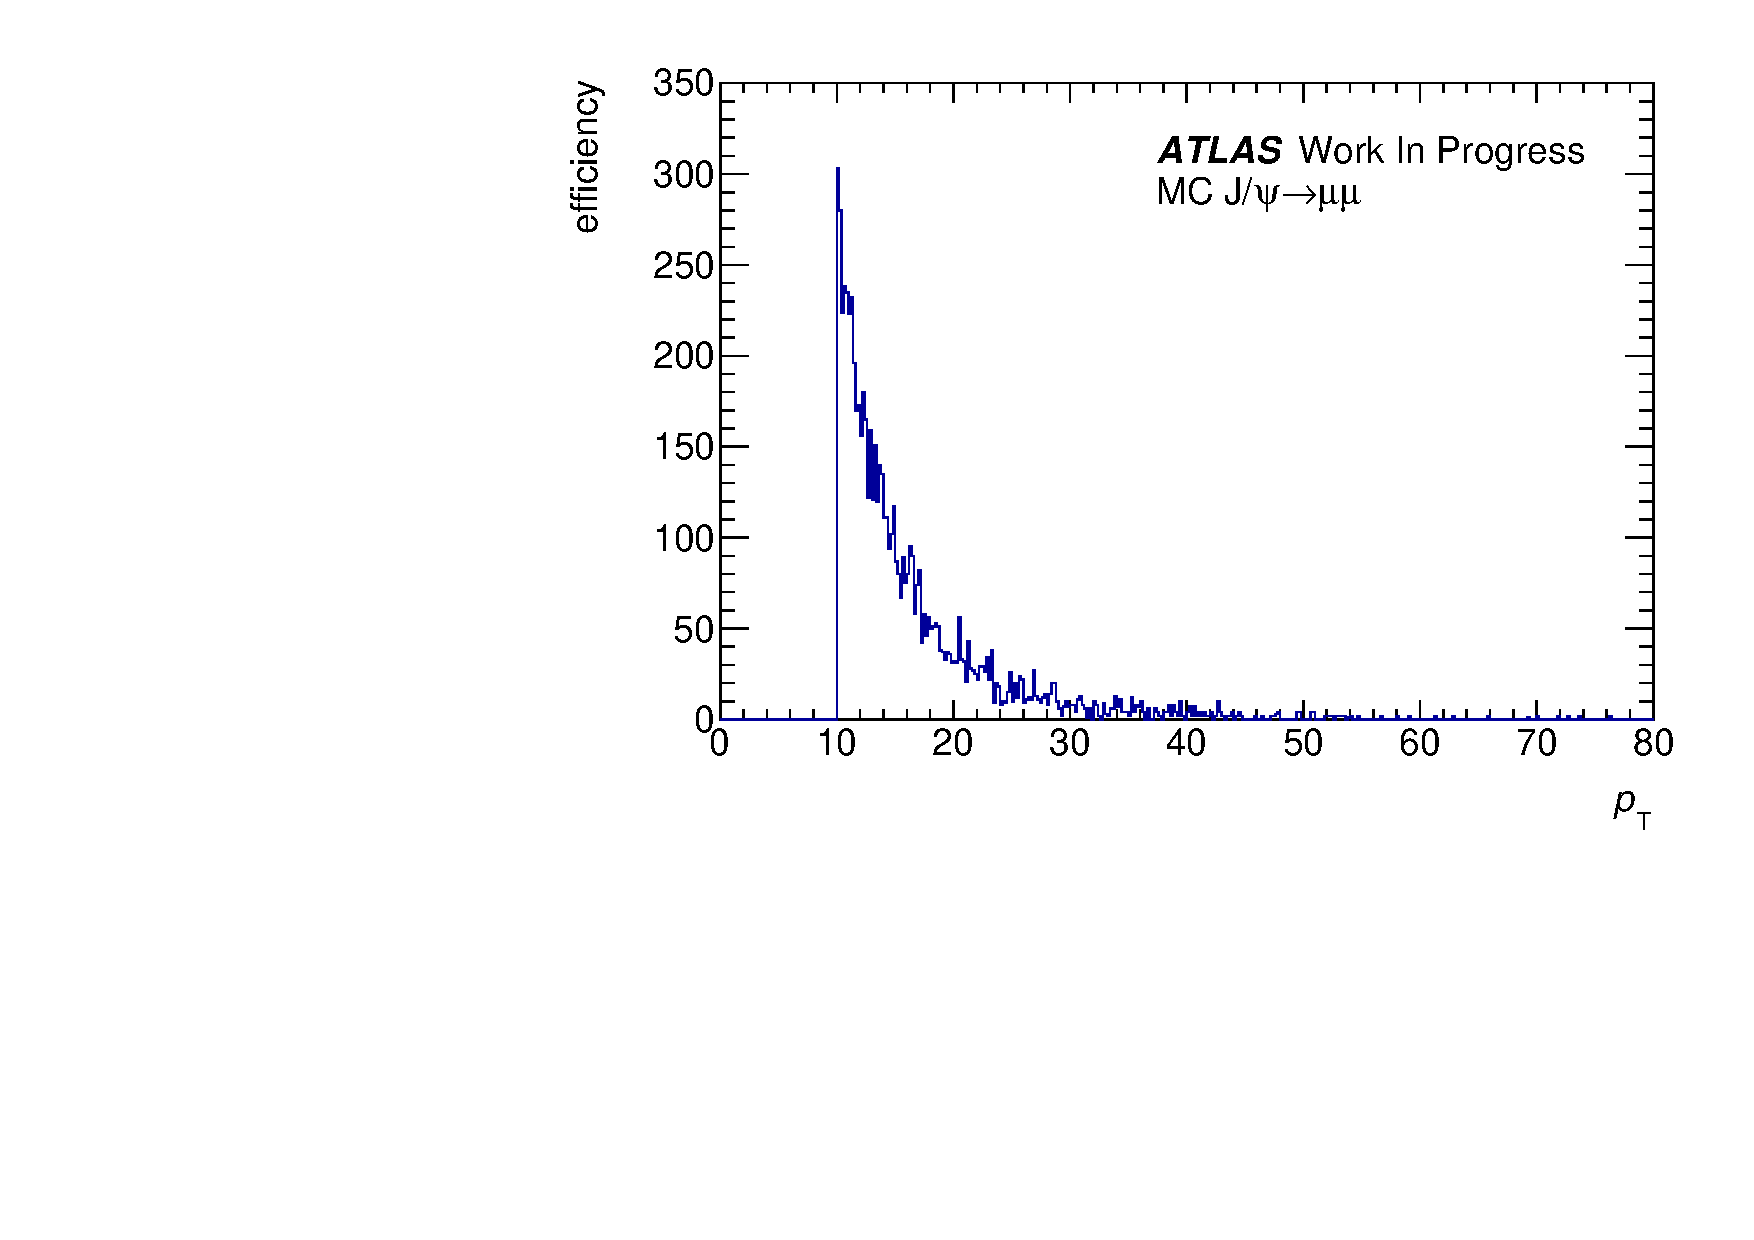
\includegraphics[clip, width=6.8cm]{fig/4/pt_MC_v2.pdf}
          \subcaption{Run-$\pt$分布}
          %\label{fig:5-8-2}
      \end{minipage} \\
      
      \begin{minipage}{0.48\linewidth}
          \centering
          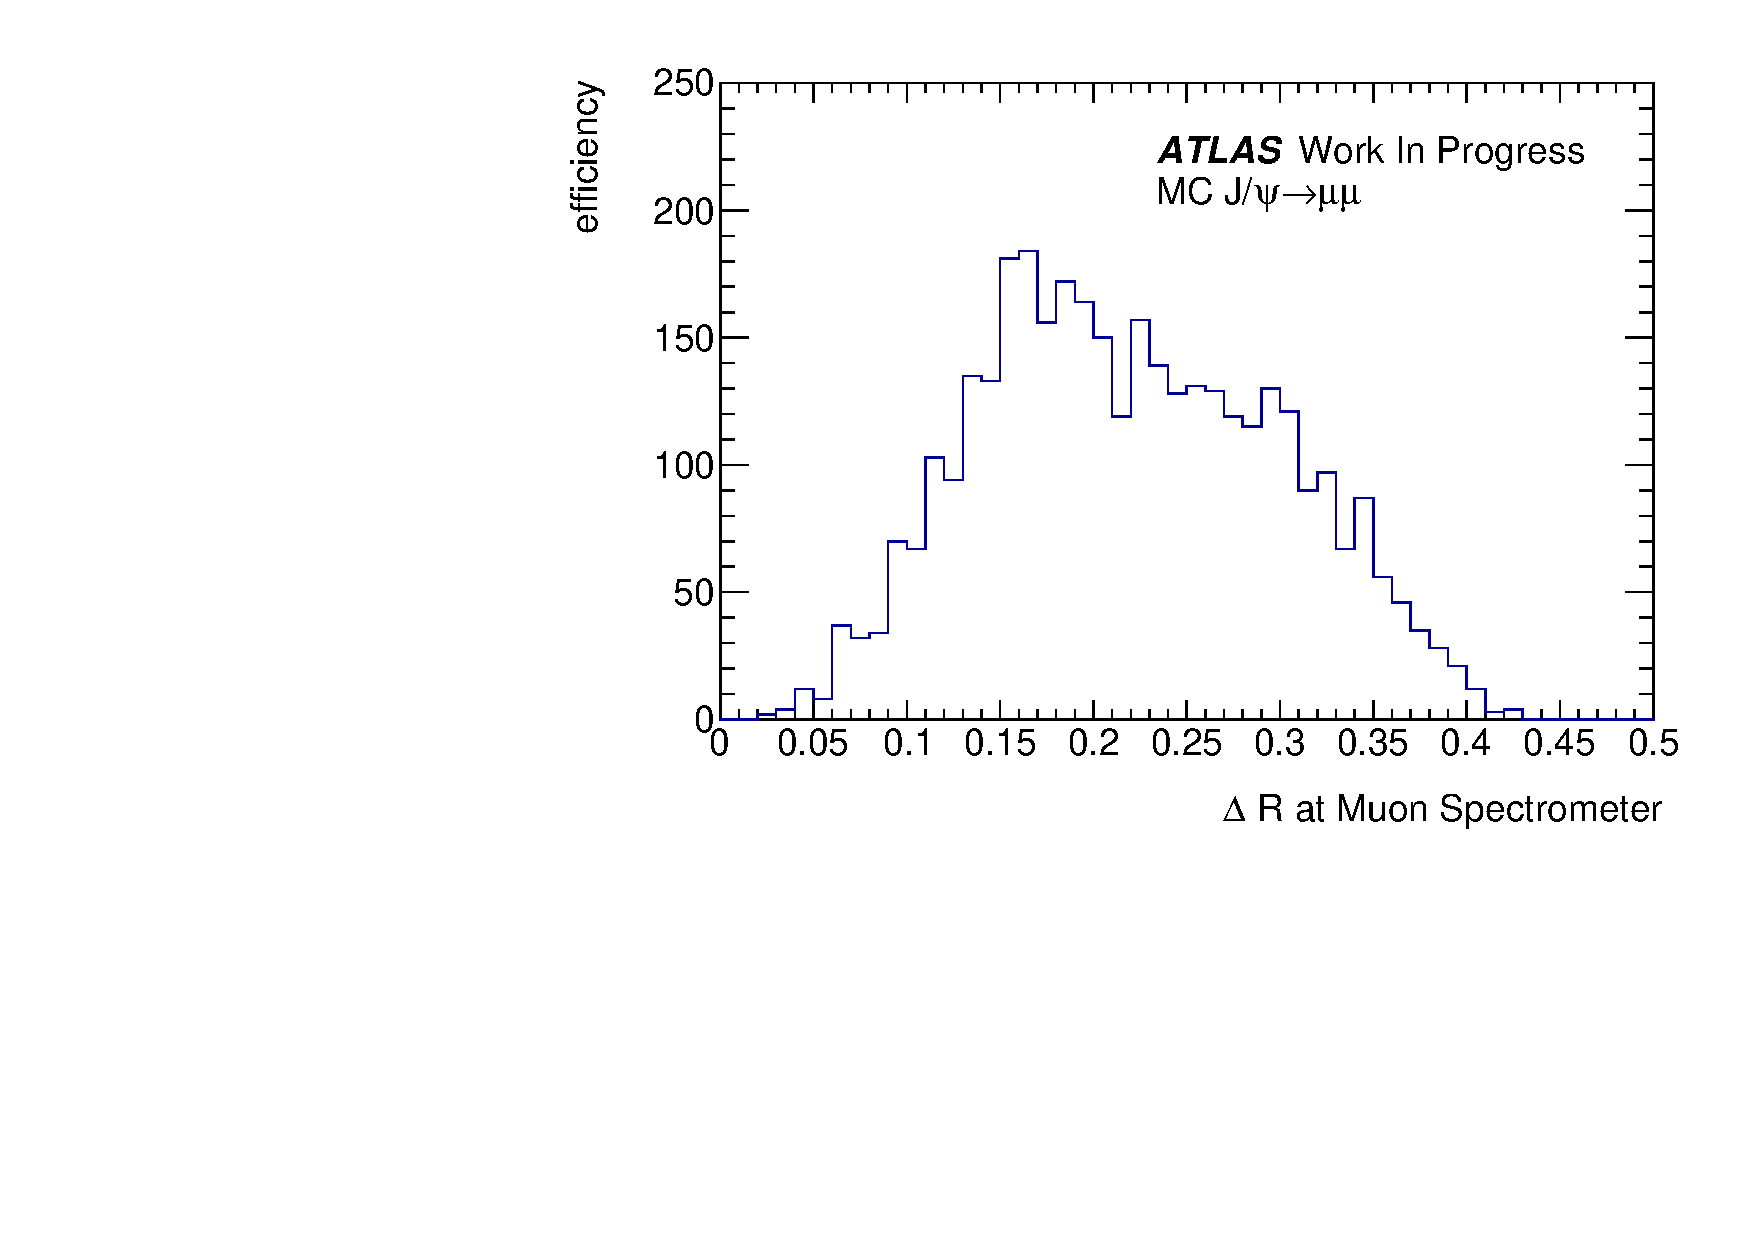
\includegraphics[clip, width=6.8cm]{fig/4/deltaR_ext_MC_v2.pdf}
          \subcaption{$\Delta R_{\mu\mu~\mathrm{at~Muon~Spectrometer}}$}
          %\label{fig:5-9-2}
      \end{minipage} \\
    \end{tabular}
    \caption{L1~BOMトリガーのトリガー効率の評価に用いたシミュレーションサンプル。}
    \label{fig:L1BOMMCSample}
\end{figure}

Run-3実データを用いて評価した~L1~BOMトリガーのトリガー効率を図~\ref{fig:L1BOMEffData}に示す。横軸は2つのミューオンのミューオン検出器での距離$\Delta R_{\mu\mu~\mathrm{at~Muon~Spectrometer}}$である。黒色が10GeV以上の$\pt$を持つミューオンを2つ要求する2ミューオントリガーのトリガー効率、赤色が10GeV以上の$\pt$を持つミューオンを1つかつ近接2ミューオンフラグを要求する~L1~BOMトリガーのトリガー効率を表す。青色が黒と赤の論理和を取った場合のトリガー効率である。

\begin{figure}[H]
    \centering
    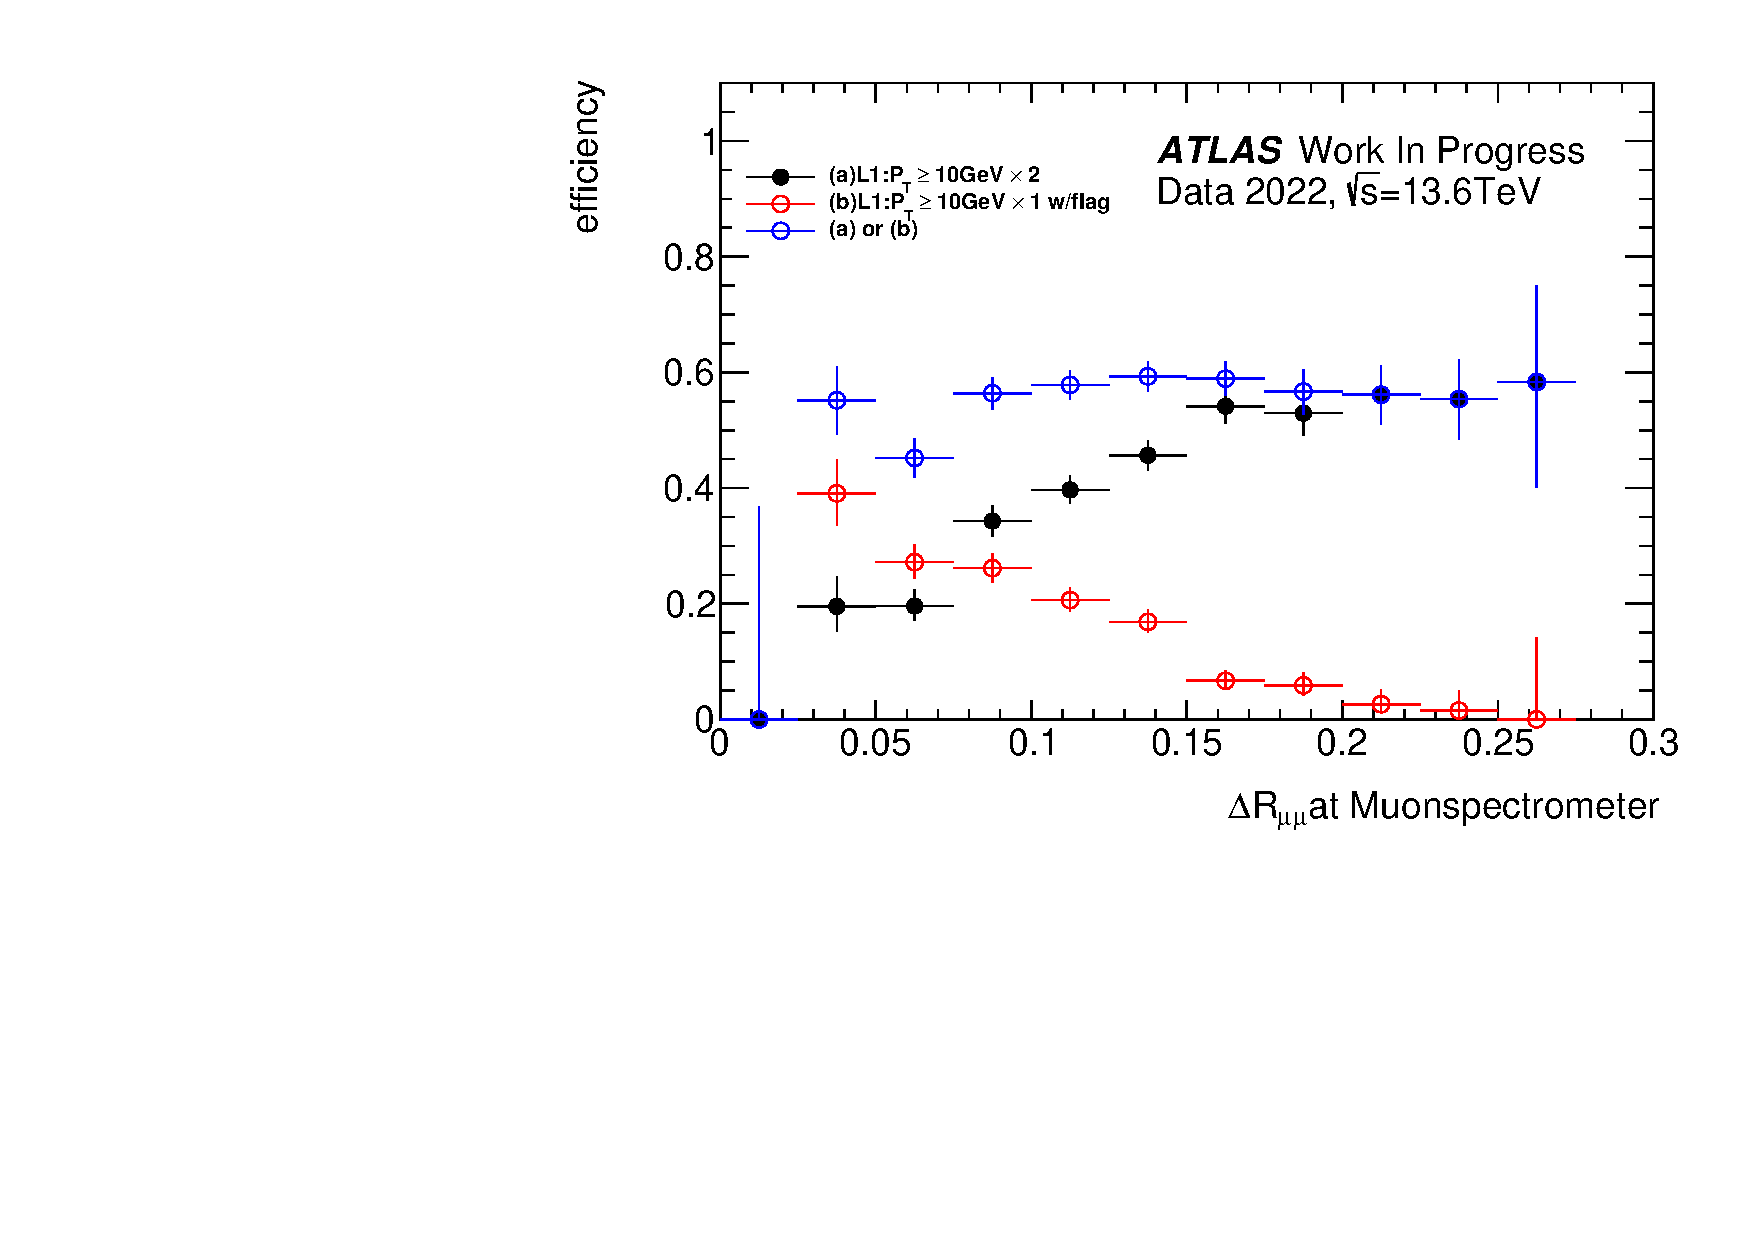
\includegraphics[clip, width=12cm]{fig/4/BOM_eff.pdf}
    \caption{L1~BOMトリガーの2022年取得~Run-3実データにおける検出効率。青点が従来の2ミューオントリガーの効率、赤点がフラグを要求したトリガーの効率、黒点が2つのトリガーの論理和を取った場合のトリガー効率。}
    \label{fig:L1BOMEffData}
\end{figure}

\begin{figure}[H]
    \centering
    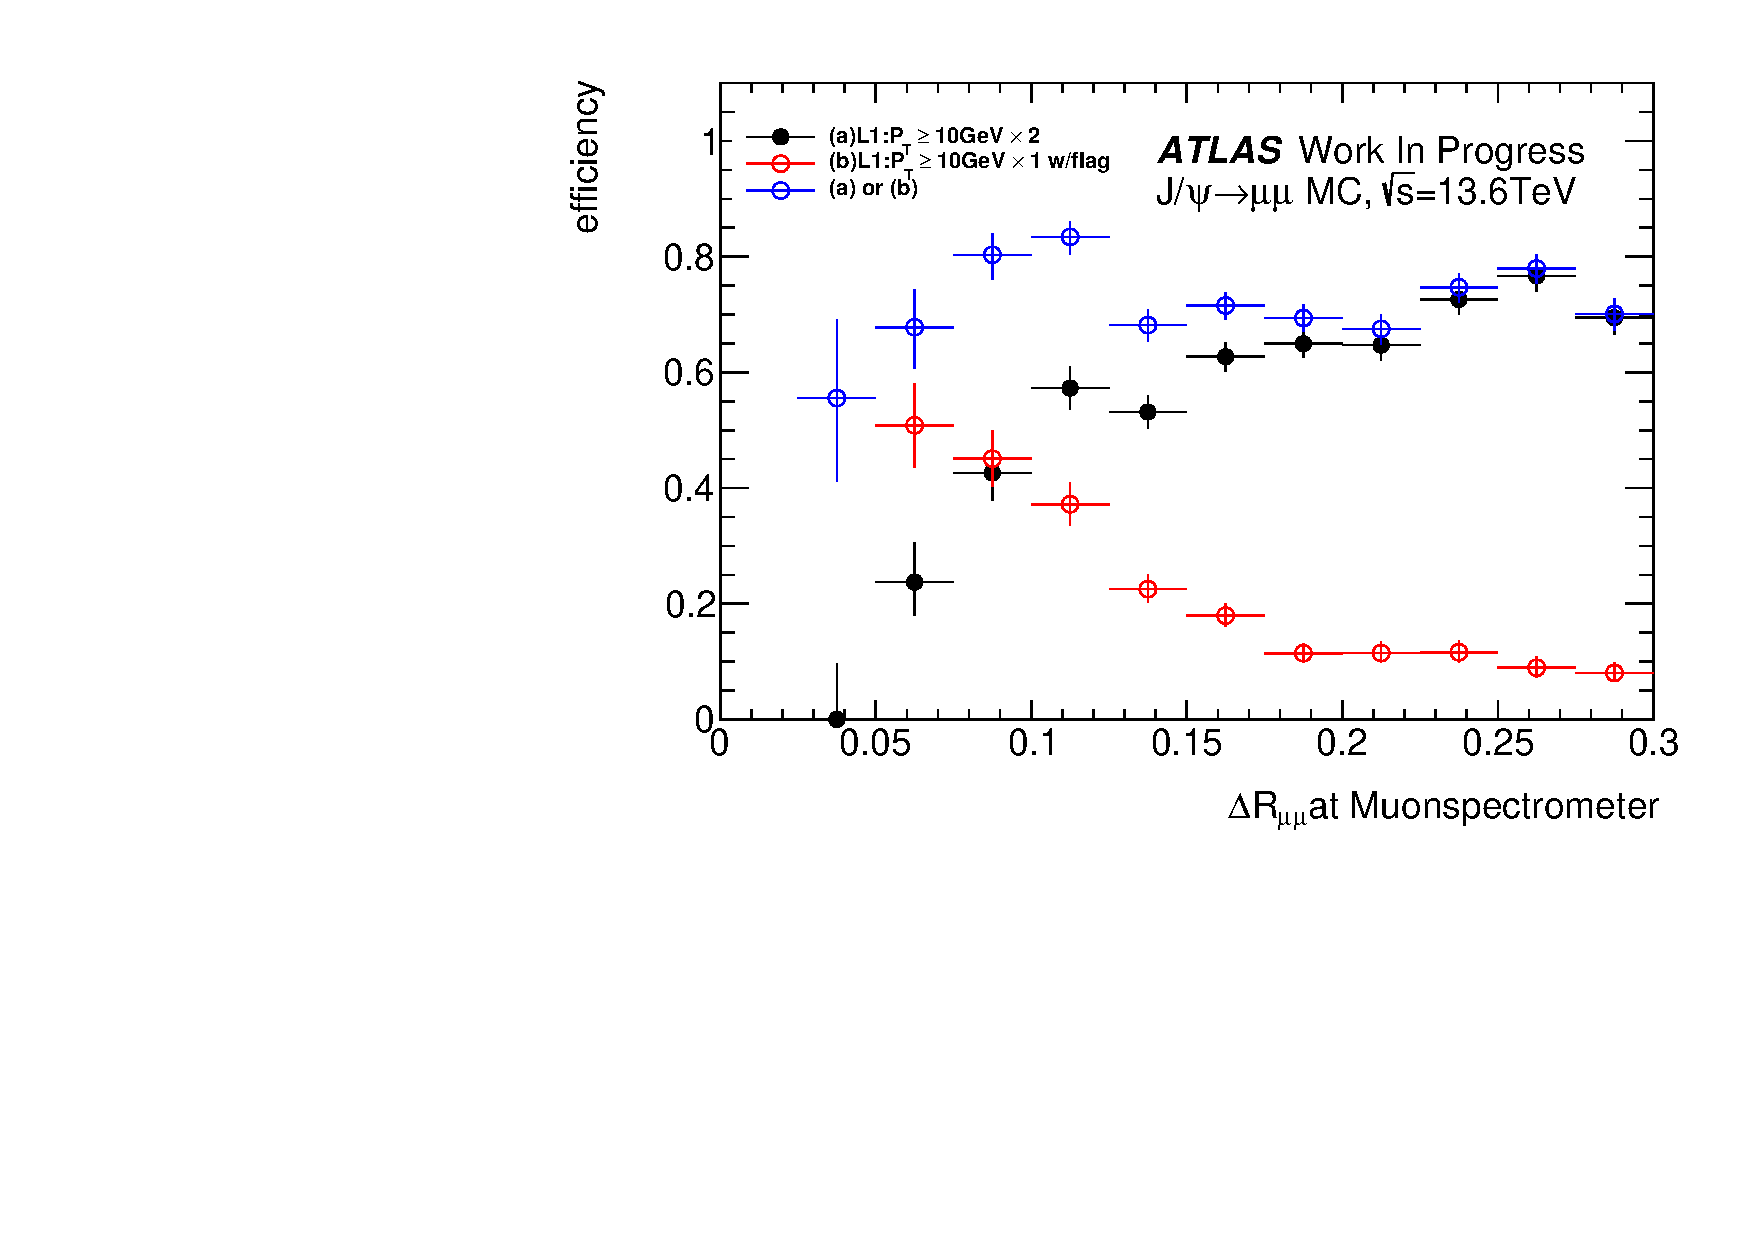
\includegraphics[clip, width=12cm]{fig/4/BOM_MC_eff.pdf}
    \caption{L1~BOMトリガーのシミュレーションにおける検出効率。赤点がフラグを要求したトリガーの効率、黒点が2つのトリガーの論理和を取った場合のトリガー効率。}
    \label{fig:L1BOMEffMC}
\end{figure}

図~\ref{fig:L1BOMEffData}から$\Delta R_{\mu\mu~\mathrm{at~Muon~Spectrometer}}<0.15$の2ミューオン同士が非常に近接している領域において、近接2ミューオンフラグを要求する~L1~BOMトリガーのトリガー効率が大きく向上している。ただし、$\Delta R_{\mu\mu~\mathrm{at~Muon~Spectrometer}}<0.03$の領域では~L1~BOMトリガーのトリガー効率も低下している。これは近接2ミューオンフラグは2つのミューオンが同一~Padの異なる~RoIを通過したときのみ立つので、同じ~RoIを通過したときは区別できないからである。2つのトリガーの論理和を取った場合、$\Delta R_{\mu\mu~\mathrm{at~Muon~Spectrometer}}>0.03$の領域で安定したトリガー効率を出せていることがわかった。
また、シミュレーションサンプルを用いて評価したトリガー効率を図~\ref{fig:L1BOMEffMC}に示す。
シミュレーションでのトリガー効率の定性的なふるまいはデータでのトリガー効率とよく一致していることがわかる。
全体的にシミュレーションでのトリガー効率に比べてデータでのトリガー効率が低いが、これは~Run-3で稼働している~ATLAS検出器において~RPCの一部のチェンバーが故障していることが主な原因であると考える。

\section{Run-3実データを用いた後段トリガーにおける近接2ミューオントリガーの動作検証}\label{chapter4-4}

mtSAのトリガー効率を評価するために用いたサンプルの不変質量$M_{\mu\mu}$と、$\pt$、$\Delta R_{\mu\mu~\mathrm{at~Muon~Spectrometer}}$分布を、実データ、シミュレーションについてそれぞれ図~\ref{fig:L2mtDataSample}、図~\ref{fig:L2mtMCSample}に示す。
L1~BOMトリガーの評価のときと同様にデータの分布は$M_{\mu\mu}$分布は条件をかけていないが、他の分布は~mtSAの効率を求める式~\ref{equ:L2mt}における分母の条件をかけている。

\begin{figure}[h]
    \begin{tabular}{cc}
      \begin{minipage}[b]{0.48\linewidth}
          \centering
          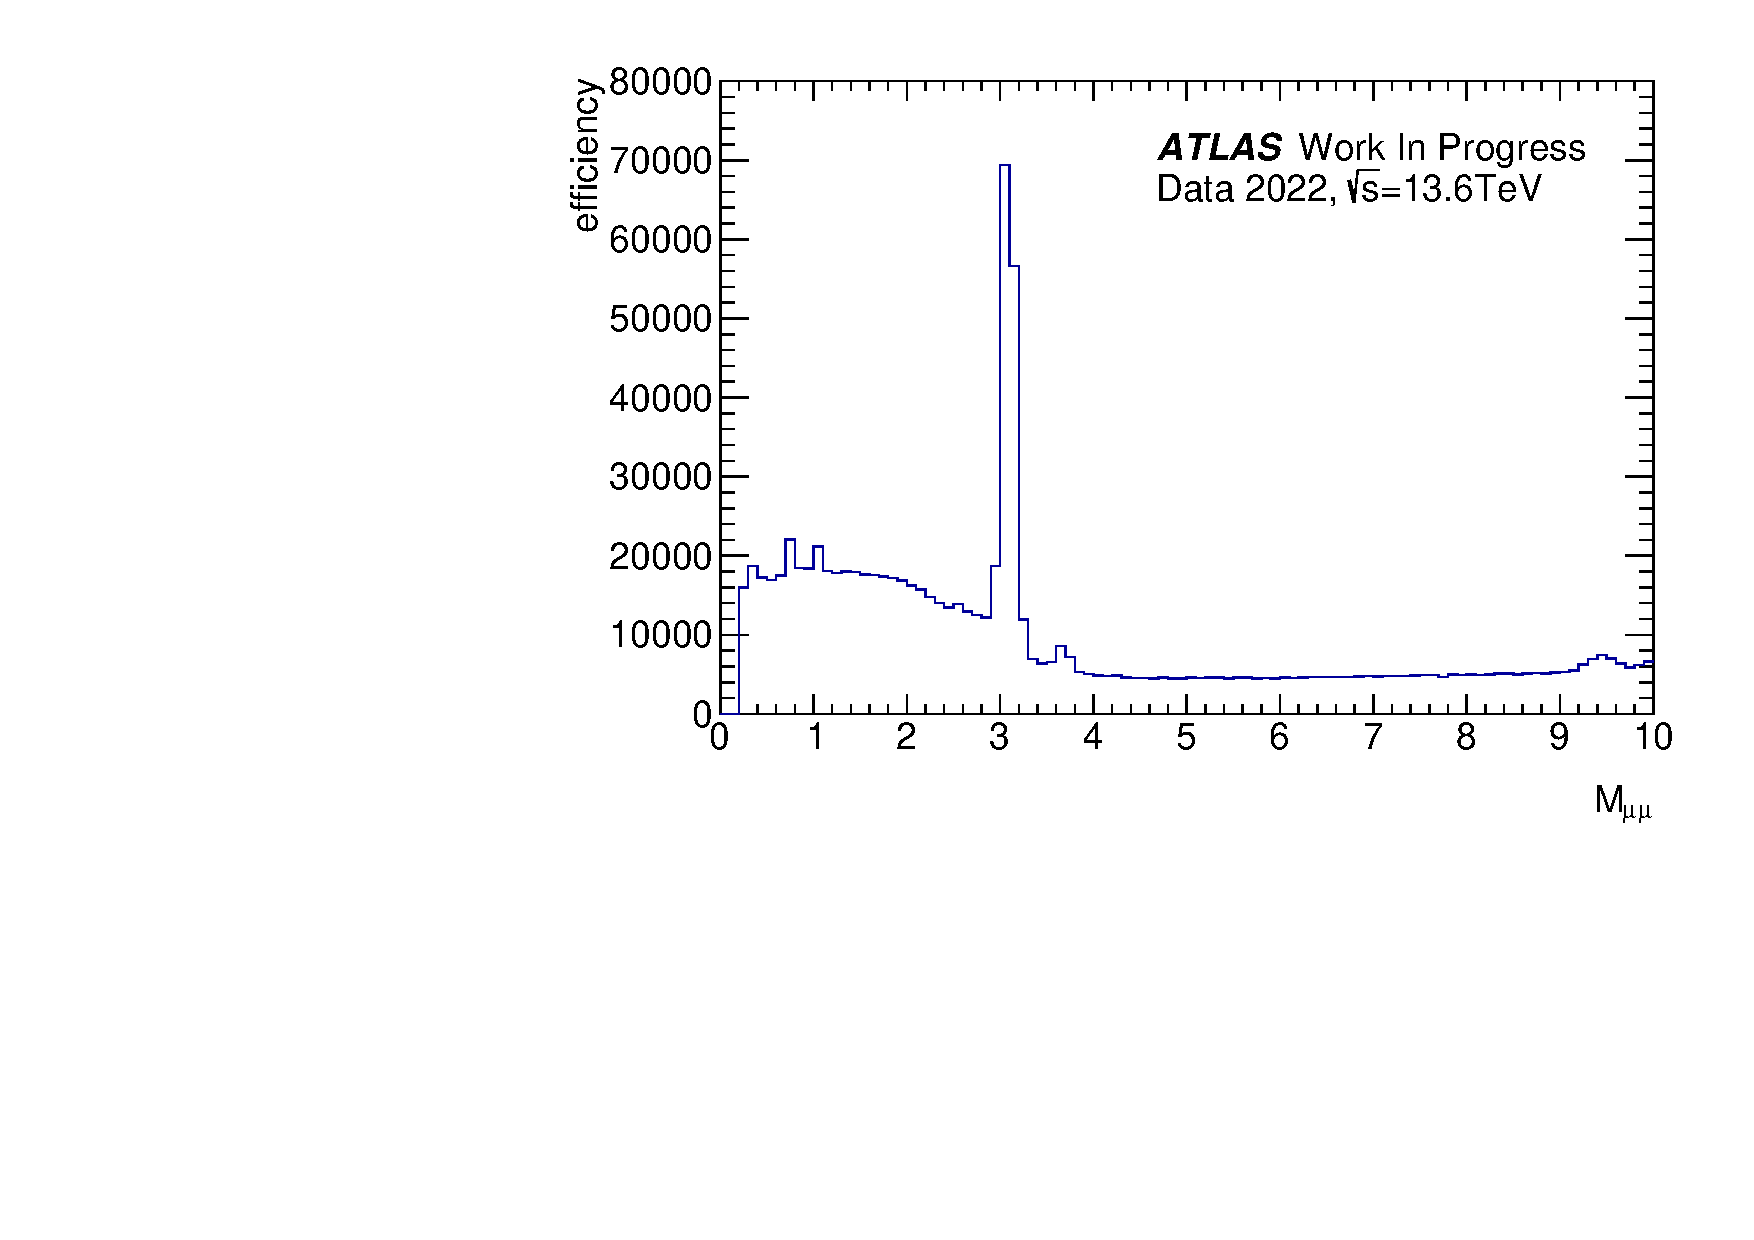
\includegraphics[clip, width=6.8cm]{fig/4/mass_data_l2mt.pdf}
          \subcaption{$M_{\mu\mu}$分布}
          %\label{fig:5-8-1}
      \end{minipage} &
      \begin{minipage}[b]{0.48\linewidth}
          \centering
          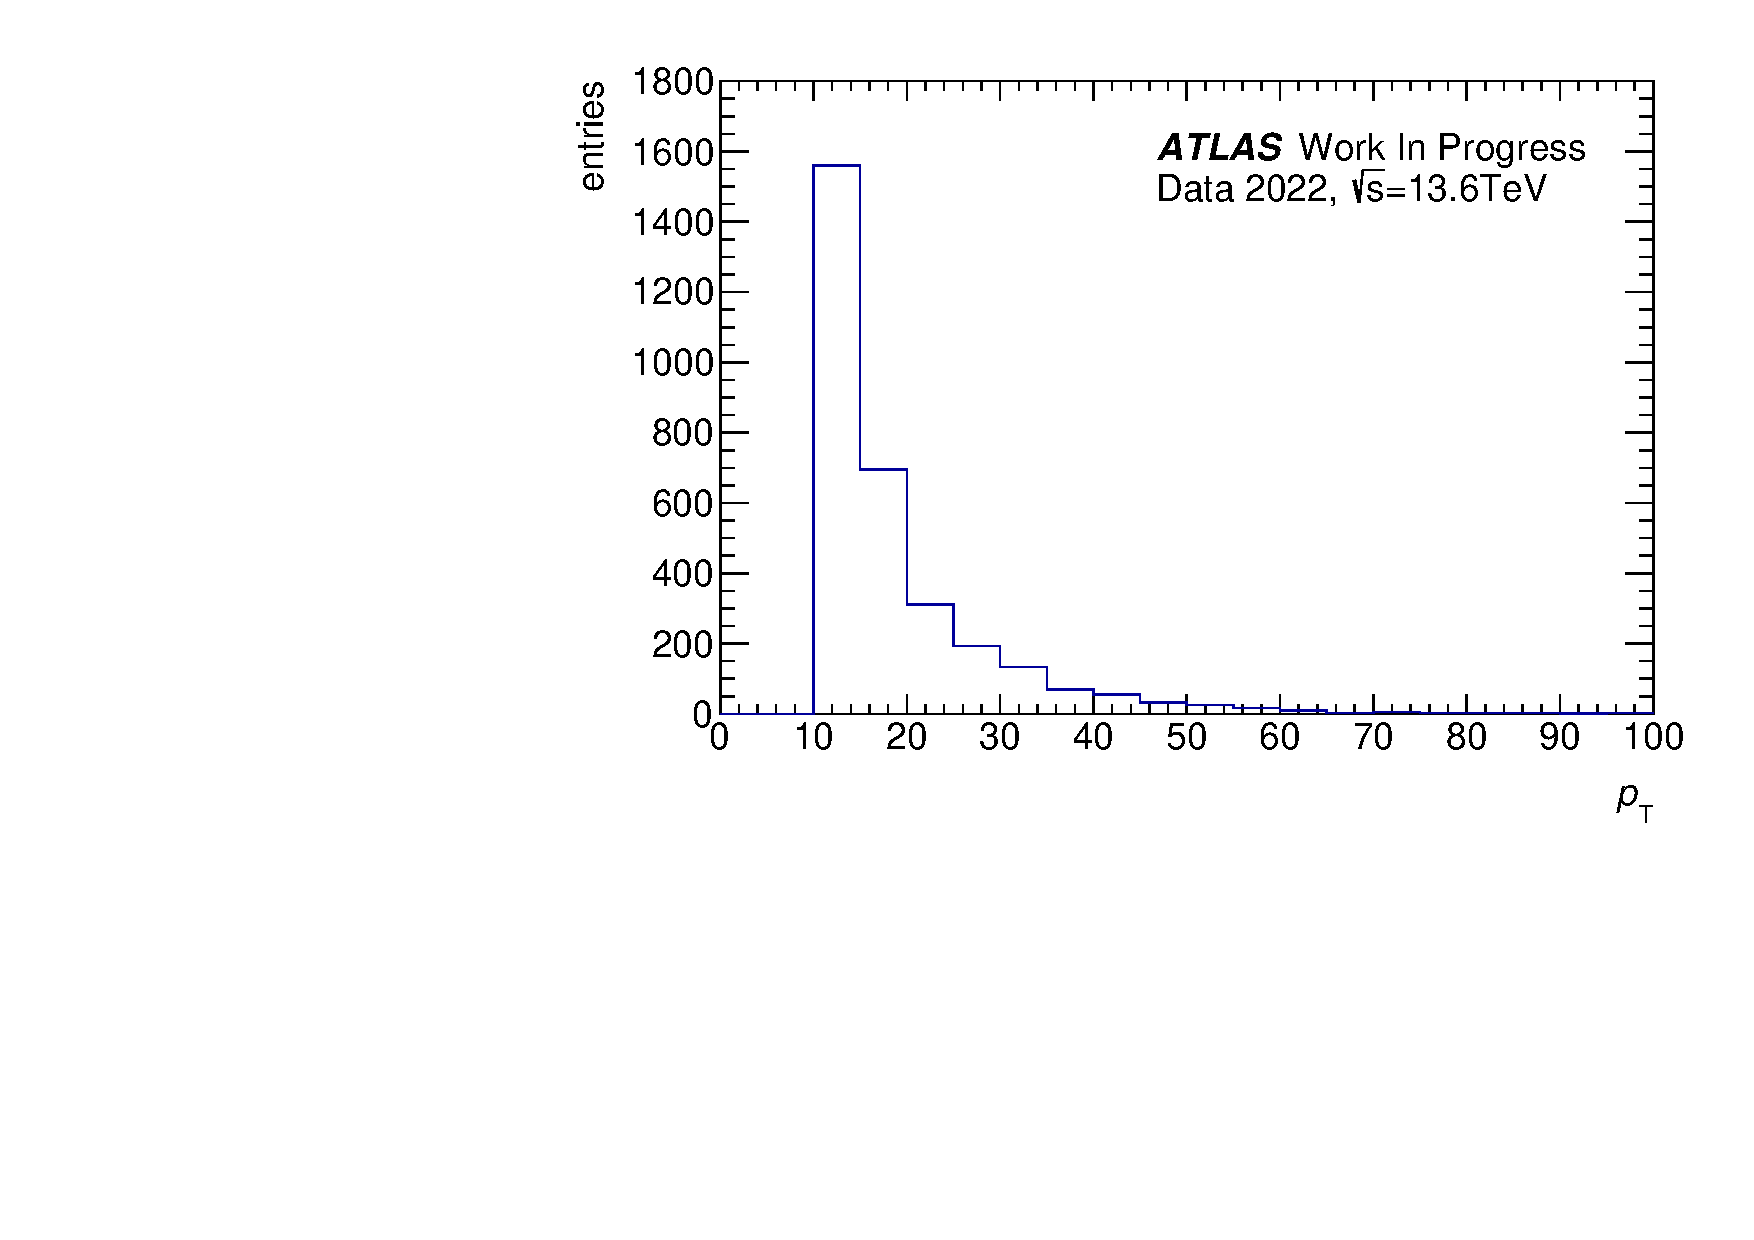
\includegraphics[clip, width=6.8cm]{fig/4/pt_data_l2mt_v2.pdf}
          \subcaption{$\pt$分布}
          %\label{fig:5-8-2}
      \end{minipage} \\
      \begin{minipage}{0.48\linewidth}
          \centering
          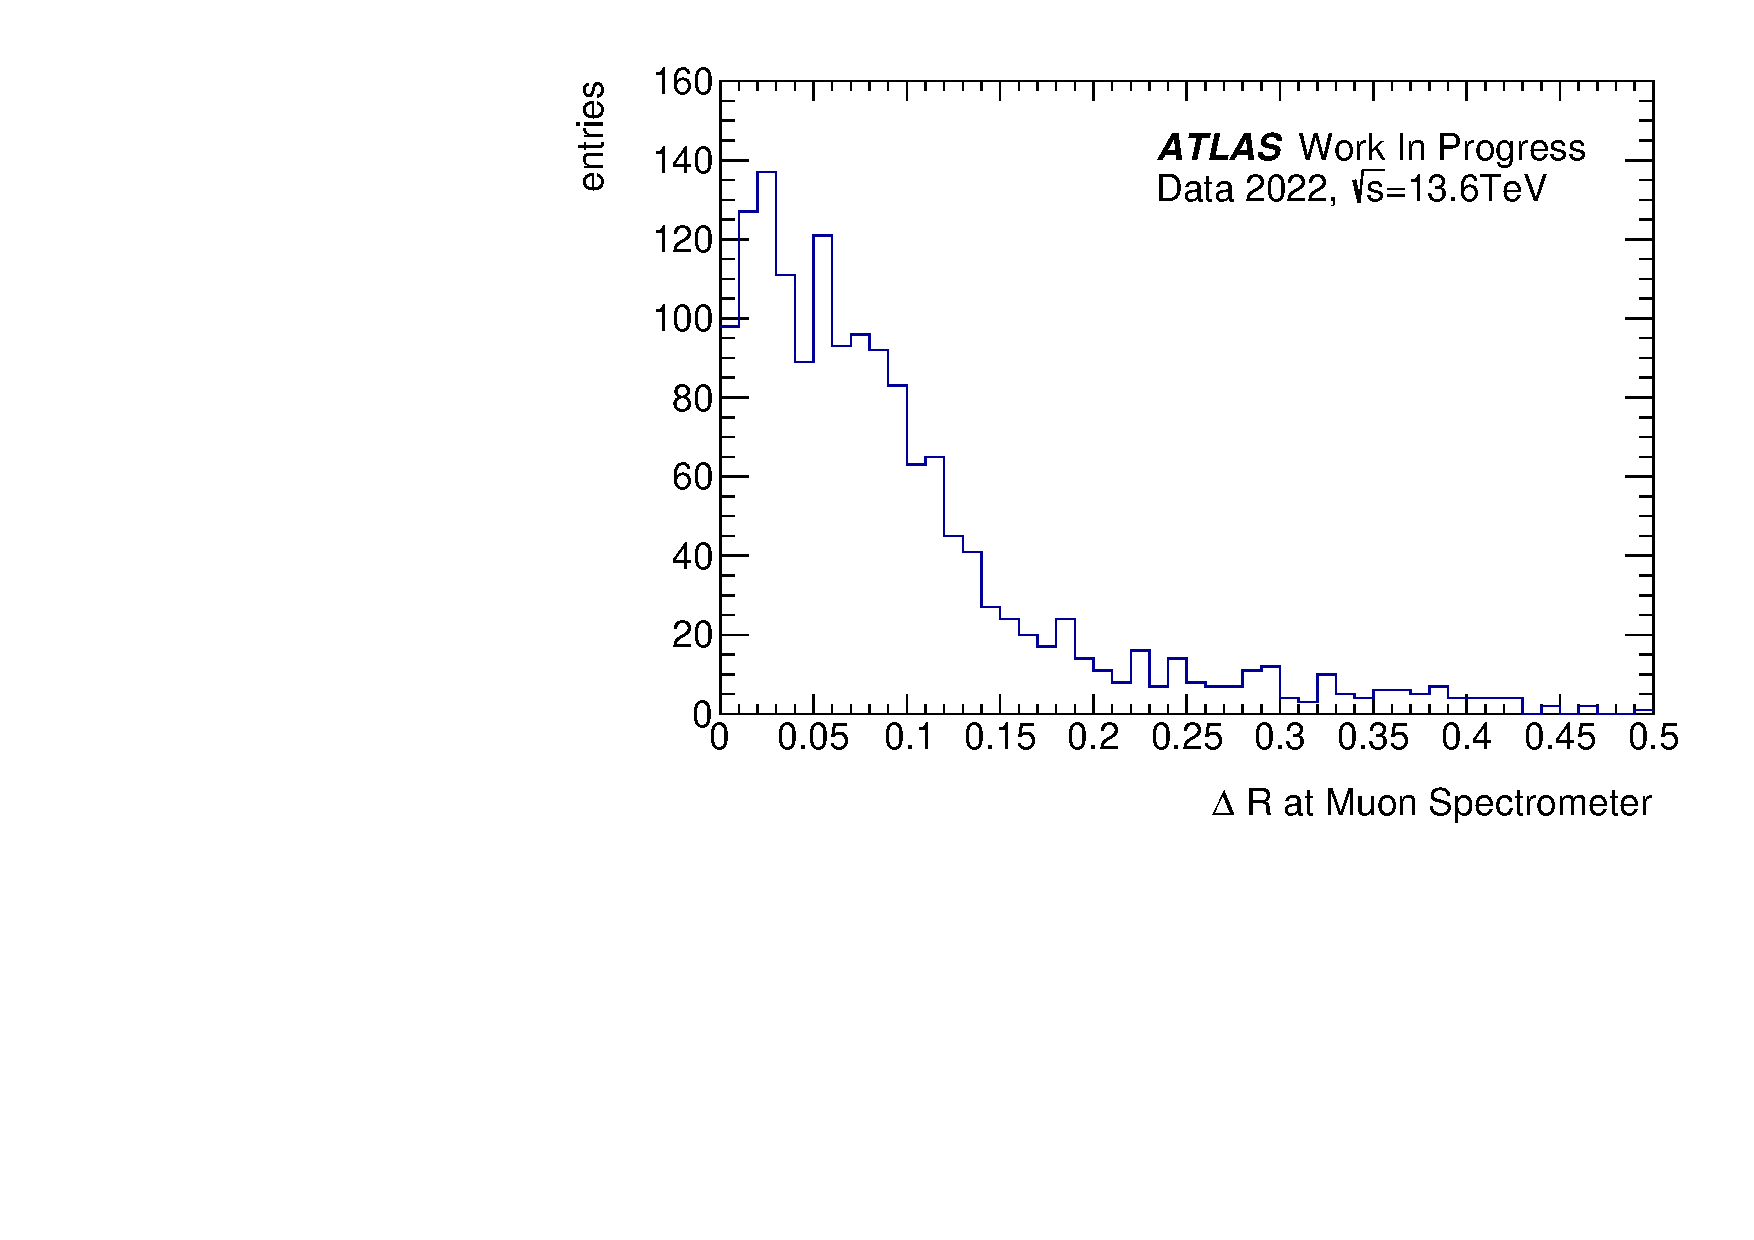
\includegraphics[clip, width=6.8cm]{fig/4/deltaR_ext_data_l2mt_v2.pdf}
          \subcaption{$\Delta R_{\mu\mu~\mathrm{at~Muon~Spectrometer}}$}
          %\label{fig:5-9-2}
      \end{minipage} \\
    \end{tabular}
    \caption{mtSAのトリガー効率の評価に用いた実データ。}
    \label{fig:L2mtDataSample}
\end{figure}

\begin{figure}[h]
    \begin{tabular}{cc}
      \begin{minipage}[b]{0.48\linewidth}
          \centering
          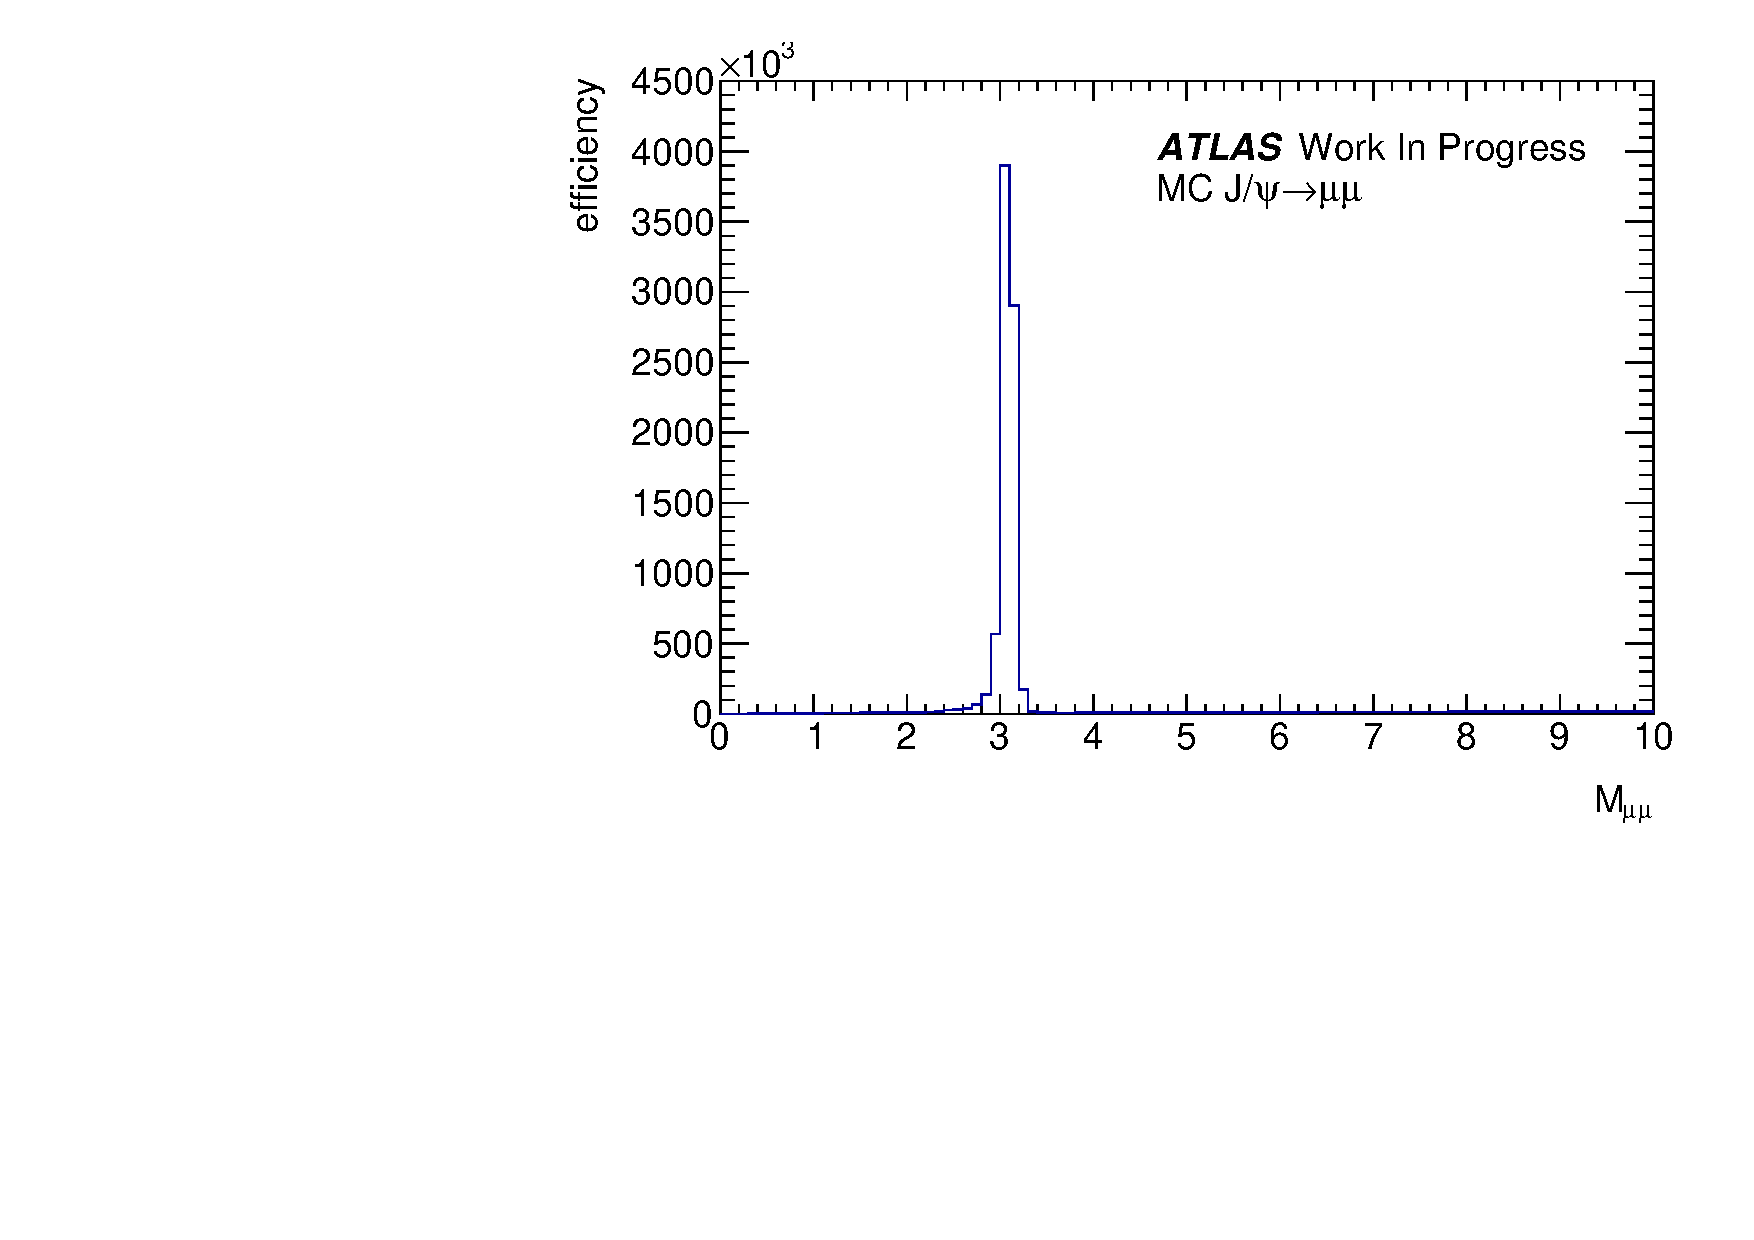
\includegraphics[clip, width=6.8cm]{fig/4/mass_MC_l2mt.pdf}
          \subcaption{Run-$M_{\mu\mu}$分布}
          %\label{fig:5-8-1}
      \end{minipage} &
      \begin{minipage}[b]{0.48\linewidth}
          \centering
          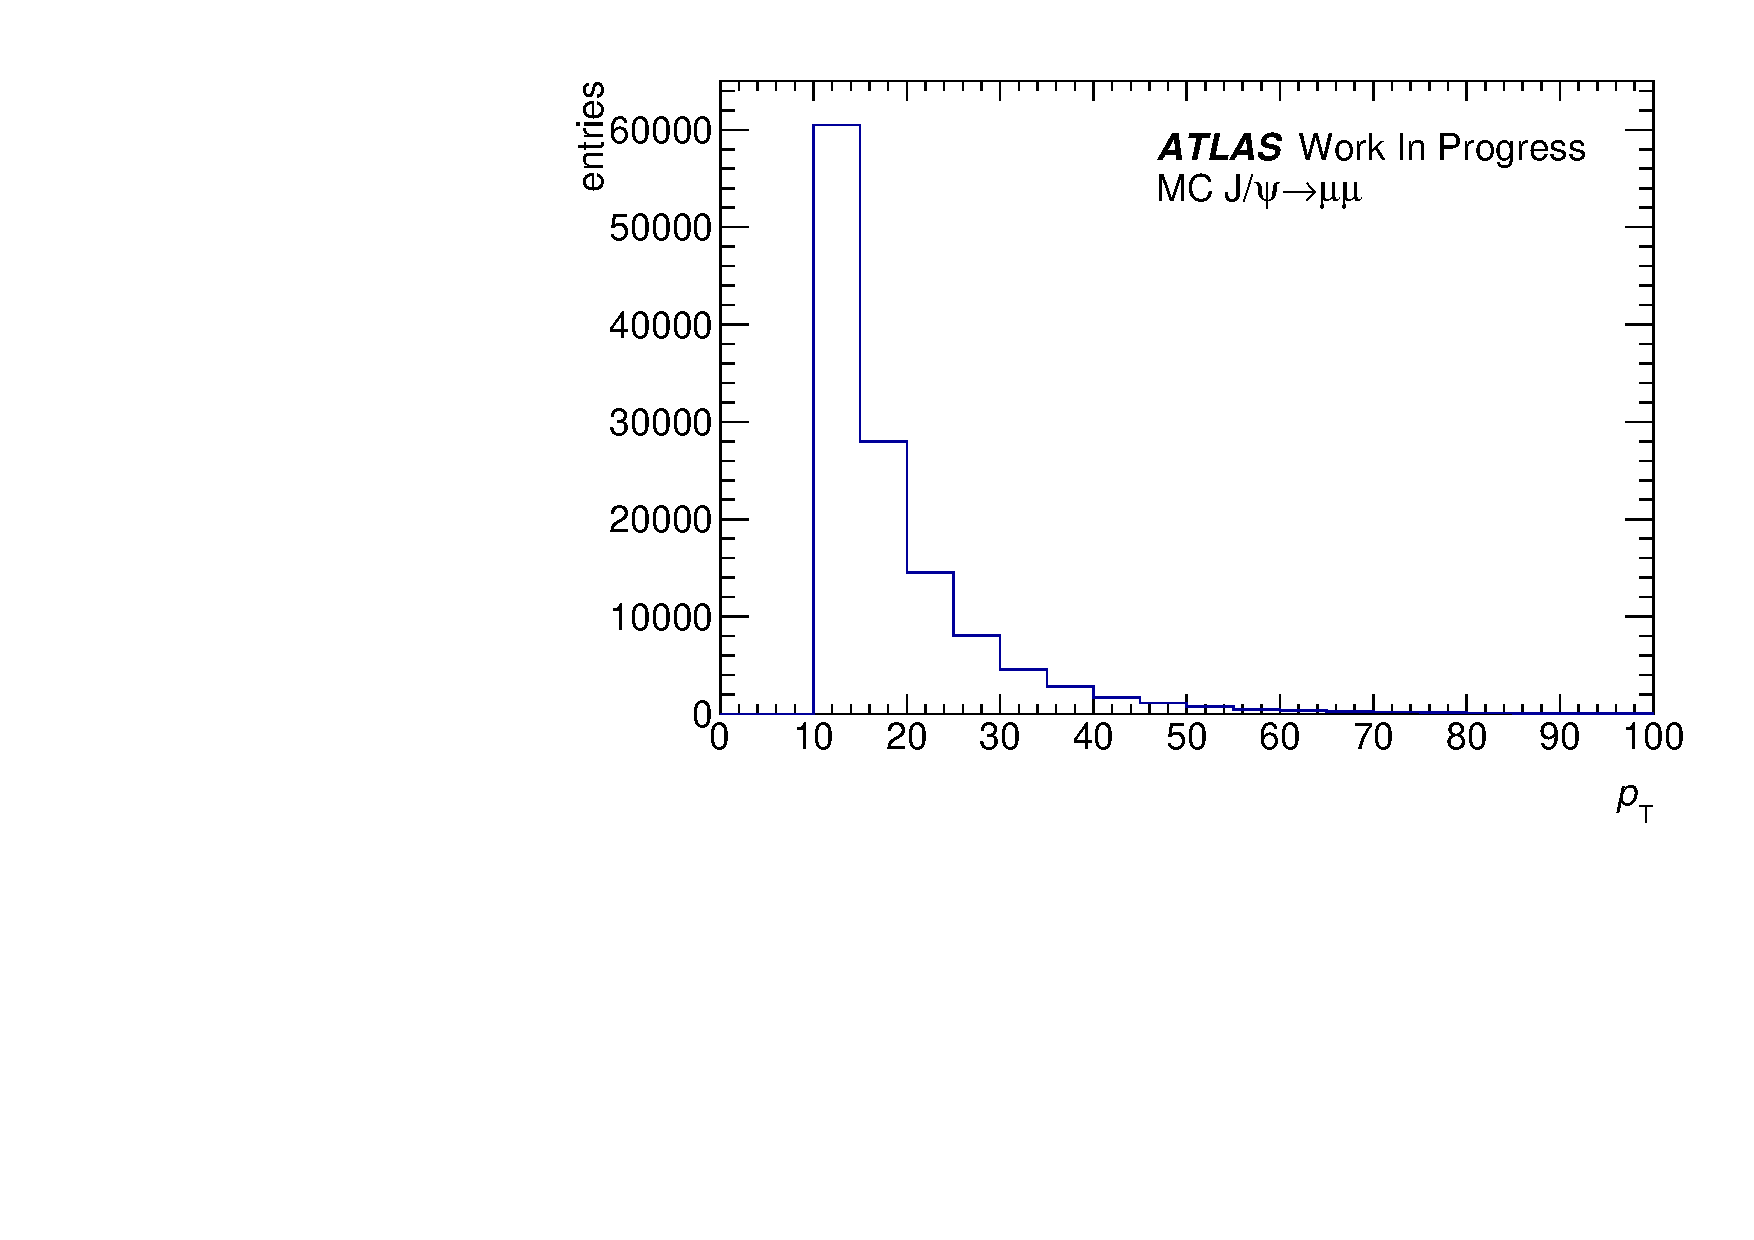
\includegraphics[clip, width=6.8cm]{fig/4/pt_MC_l2mt_v2.pdf}
          \subcaption{Run-$\pt$分布}
          %\label{fig:5-8-2}
      \end{minipage} \\
      \begin{minipage}{0.48\linewidth}
          \centering
          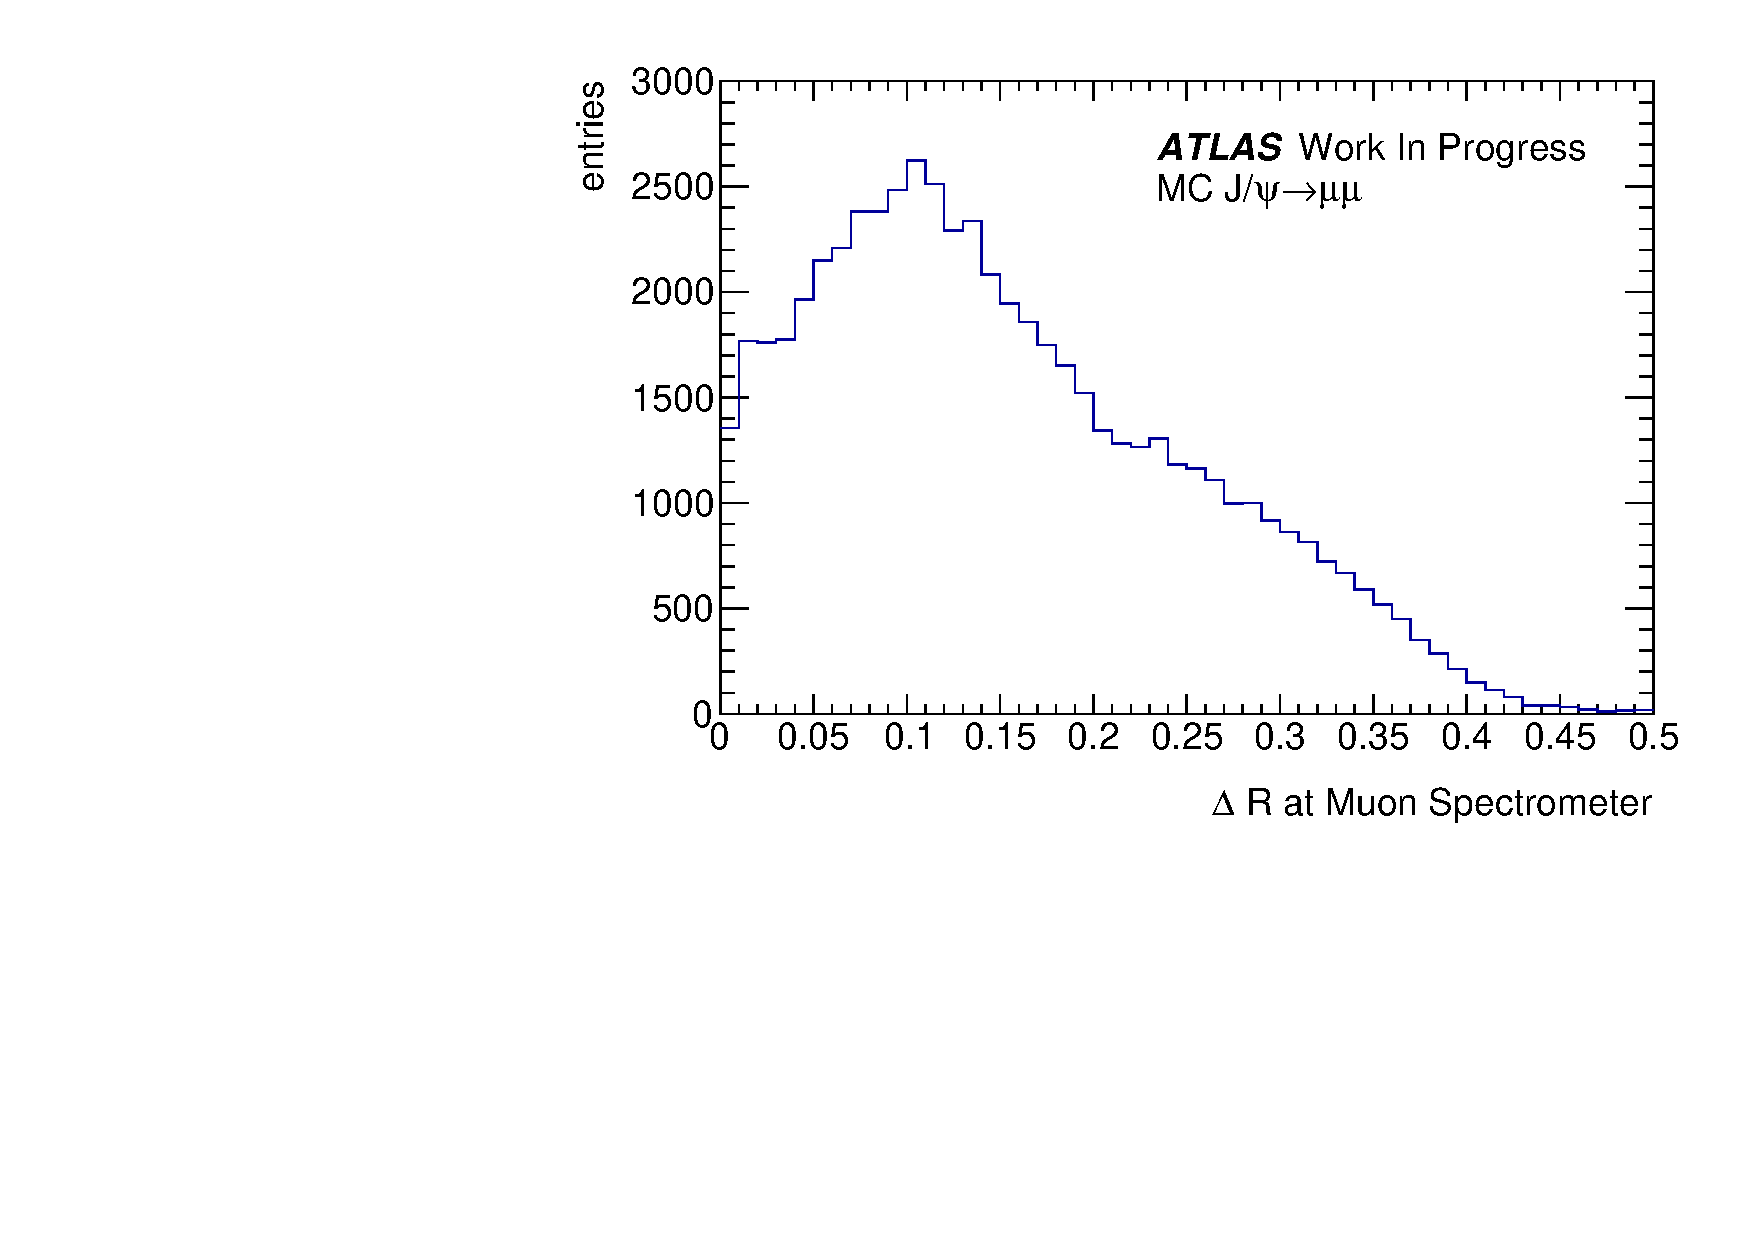
\includegraphics[clip, width=6.8cm]{fig/4/deltaR_ext_MC_l2mt_v2.pdf}
          \subcaption{$\Delta R_{\mu\mu~\mathrm{at~Muon~Spectrometer}}$}
          %\label{fig:5-9-2}
      \end{minipage} \\
    \end{tabular}
    \caption{mtSAのトリガー効率の評価に用いたシミュレーションサンプル。}
    \label{fig:L2mtMCSample}
\end{figure}

\begin{figure}[h]
    \centering
    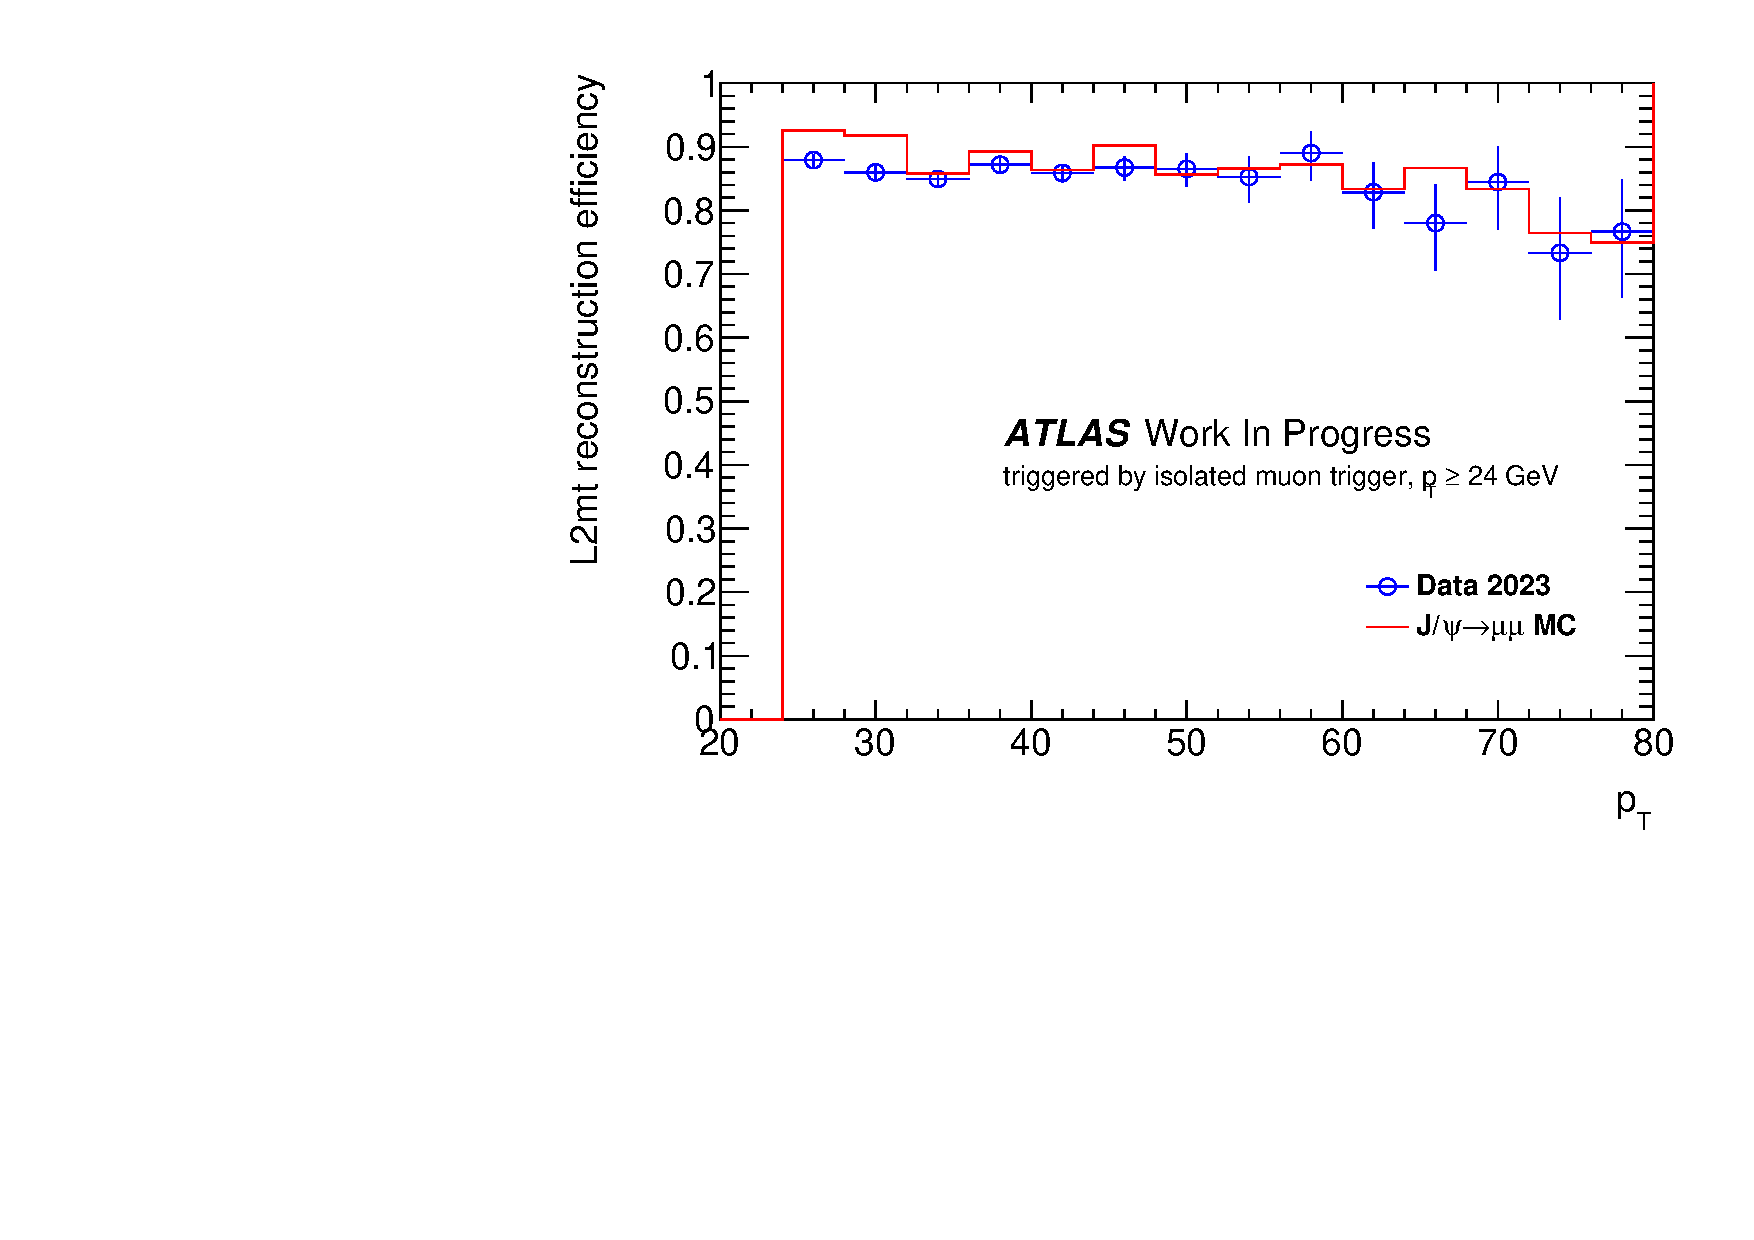
\includegraphics[clip, width=12cm]{fig/4/L2mt_singlemuon_eff.pdf}
    \caption{mtSAのシングルミューオントリガーとしての検出効率。赤線がシミュレーションでの結果、青点がデータでの結果。}
    \label{fig:L2mtSingleEff}
\end{figure}

\begin{figure}[h]
    \centering
    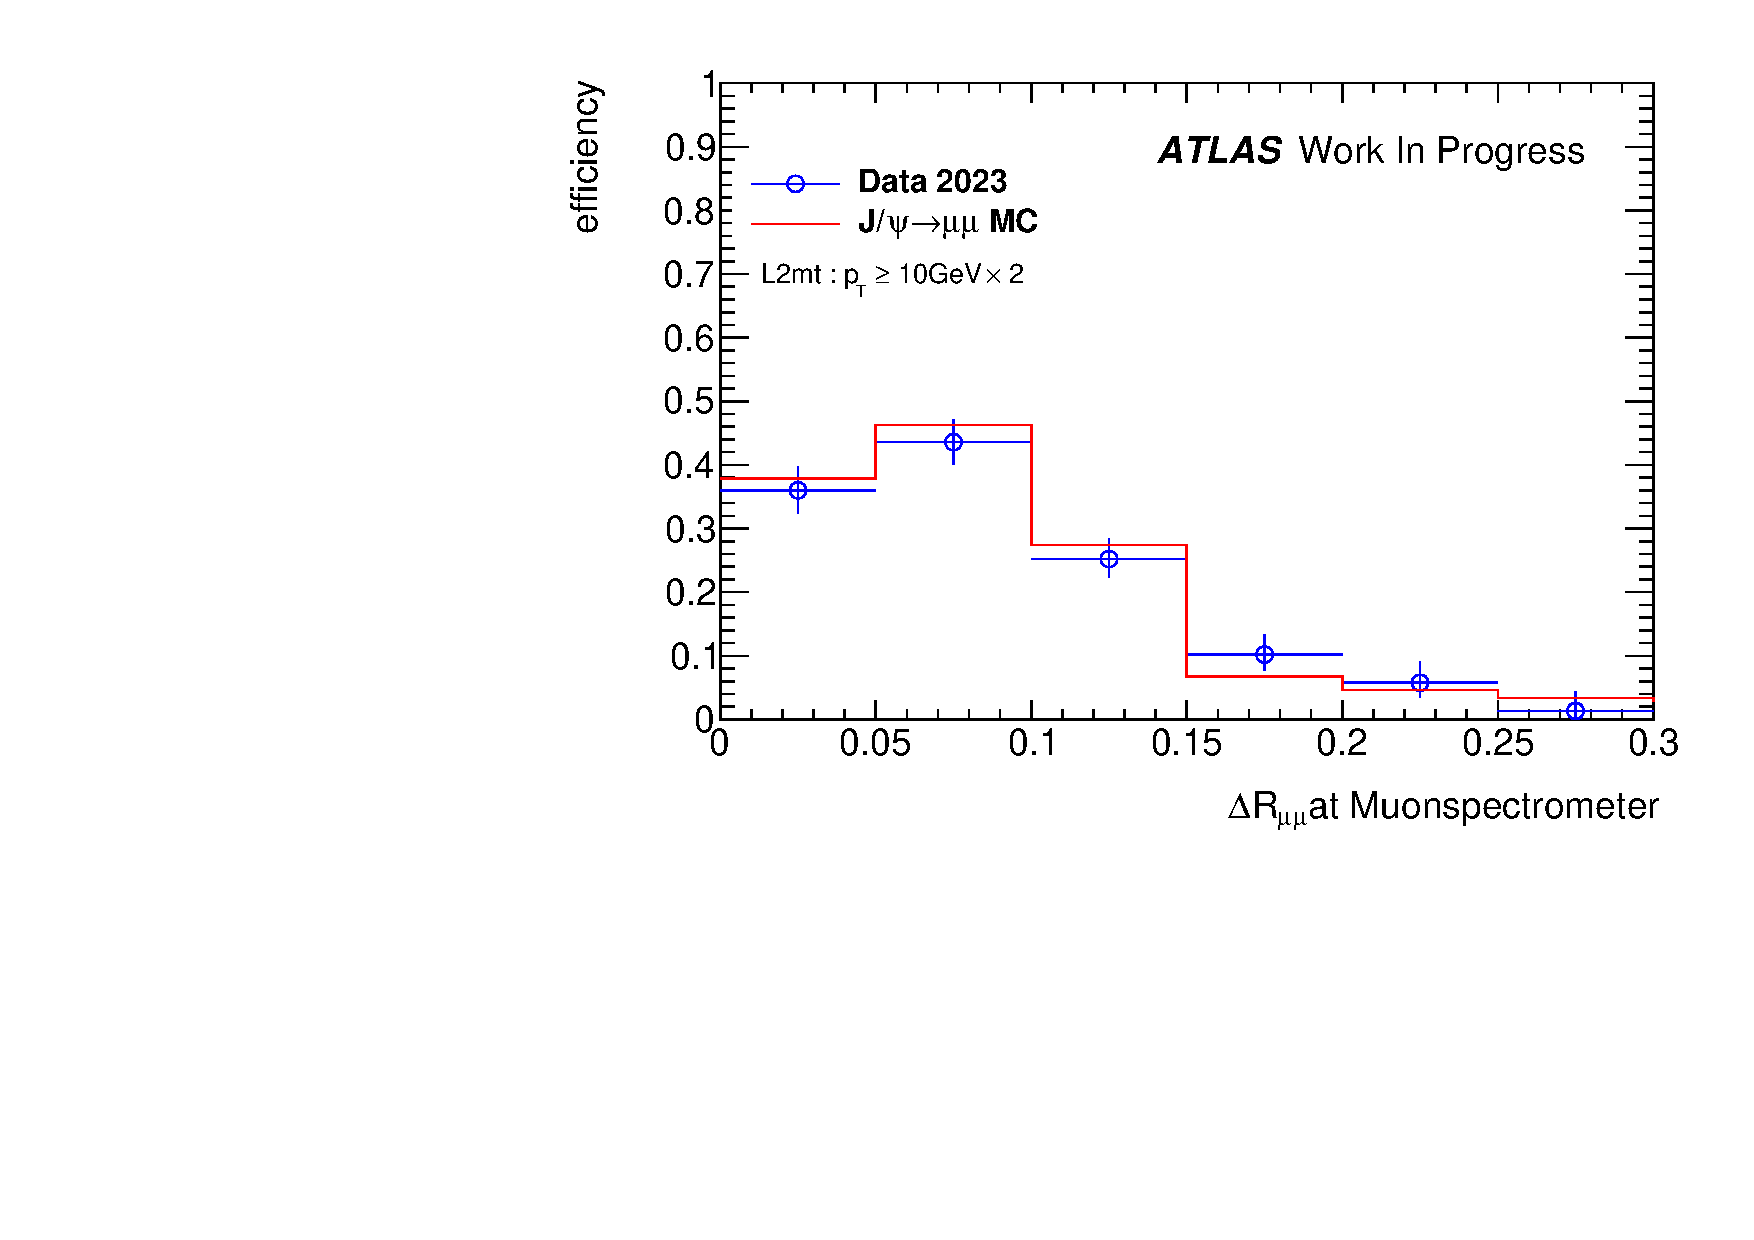
\includegraphics[clip, width=12cm]{fig/4/L2mt_eff_ext_deltaR.pdf}
    \caption{mtSAの2つ目を見つける効率。赤線がシミュレーションでの結果、青点がデータでの結果。}
    \label{fig:L2mt2muonEff}
\end{figure}

mtSAのシングルミューオントリガーとしての効率を図~\ref{fig:L2mtSingleEff}に、mtSAが2つ目のミューオンを再構成する効率を図~\ref{fig:L2mt2muonEff}に示す。
それぞれの図において、赤線がシミュレーション、青色の点がデータから求めた検出効率である。
どちらのトリガー効率も、データでのトリガー効率とシミュレーションでのトリガー効率は概ね一致している。
mtSAでのシングルミューオンの検出効率は~L2MuonSAではほぼ100$\%$であるのに対して、全体で90$\%$程度であるが、これはシミュレーションから求めた結果と一致する。

2ミューオンに対しての~mtSAの効率を図~\ref{fig:L2mt2muonEff}に示す。
mtSAが2つ目のミューオンを再構成する割合が、従来のL2MuonSAでトリガー効率が低下していた$\Delta R_{\mu\mu~\mathrm{at~Muon~Spectrometer}}<0.15$の領域において向上していることがわかった。

\begin{figure}[h]
    \centering
    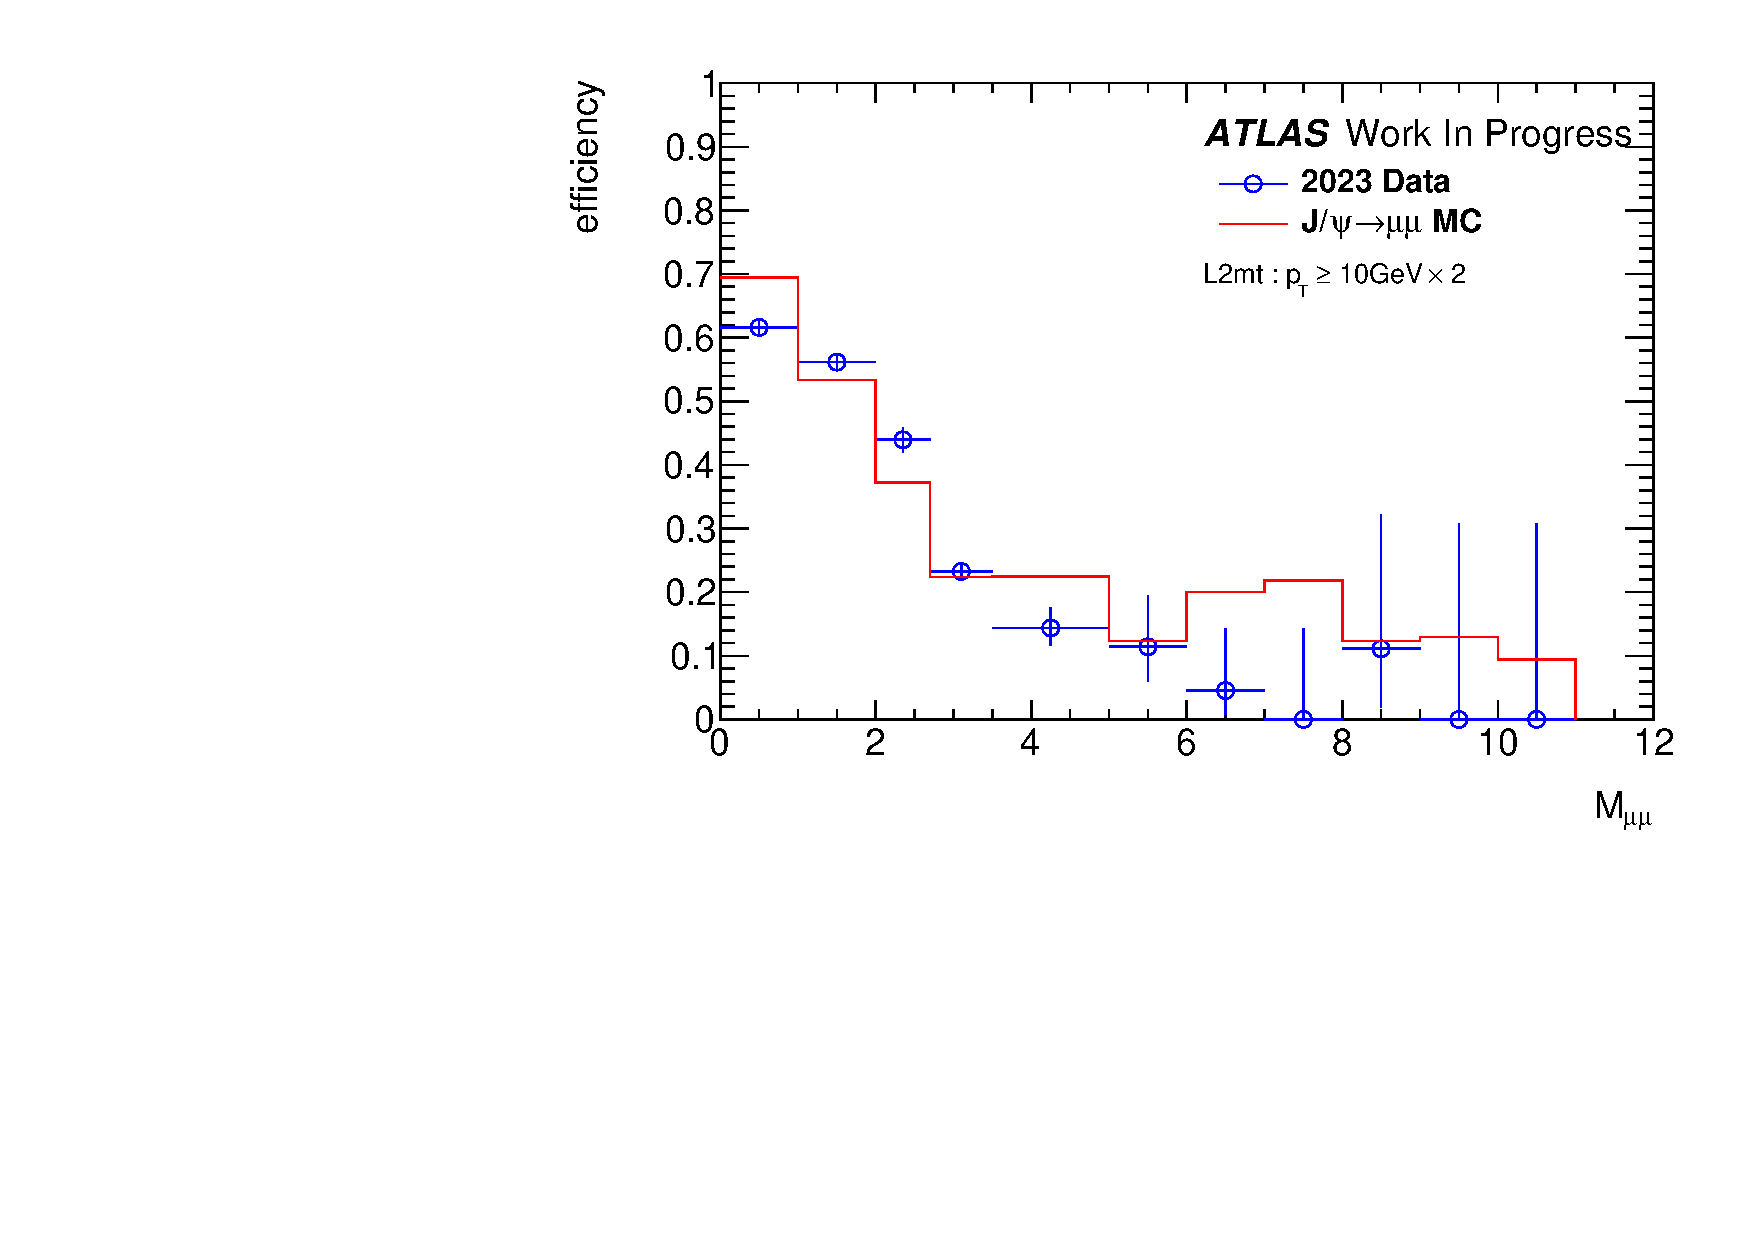
\includegraphics[clip, width=12cm]{fig/4/L2mt_eff_mass.pdf}
    \caption{横軸が2ミューオンの不変質量でのmtSAの2つ目を見つける効率。赤線がシミュレーションでの結果、青点がデータでの結果。}
    \label{fig:L2mtMassEff}
\end{figure}

\begin{figure}[h]
    \centering
    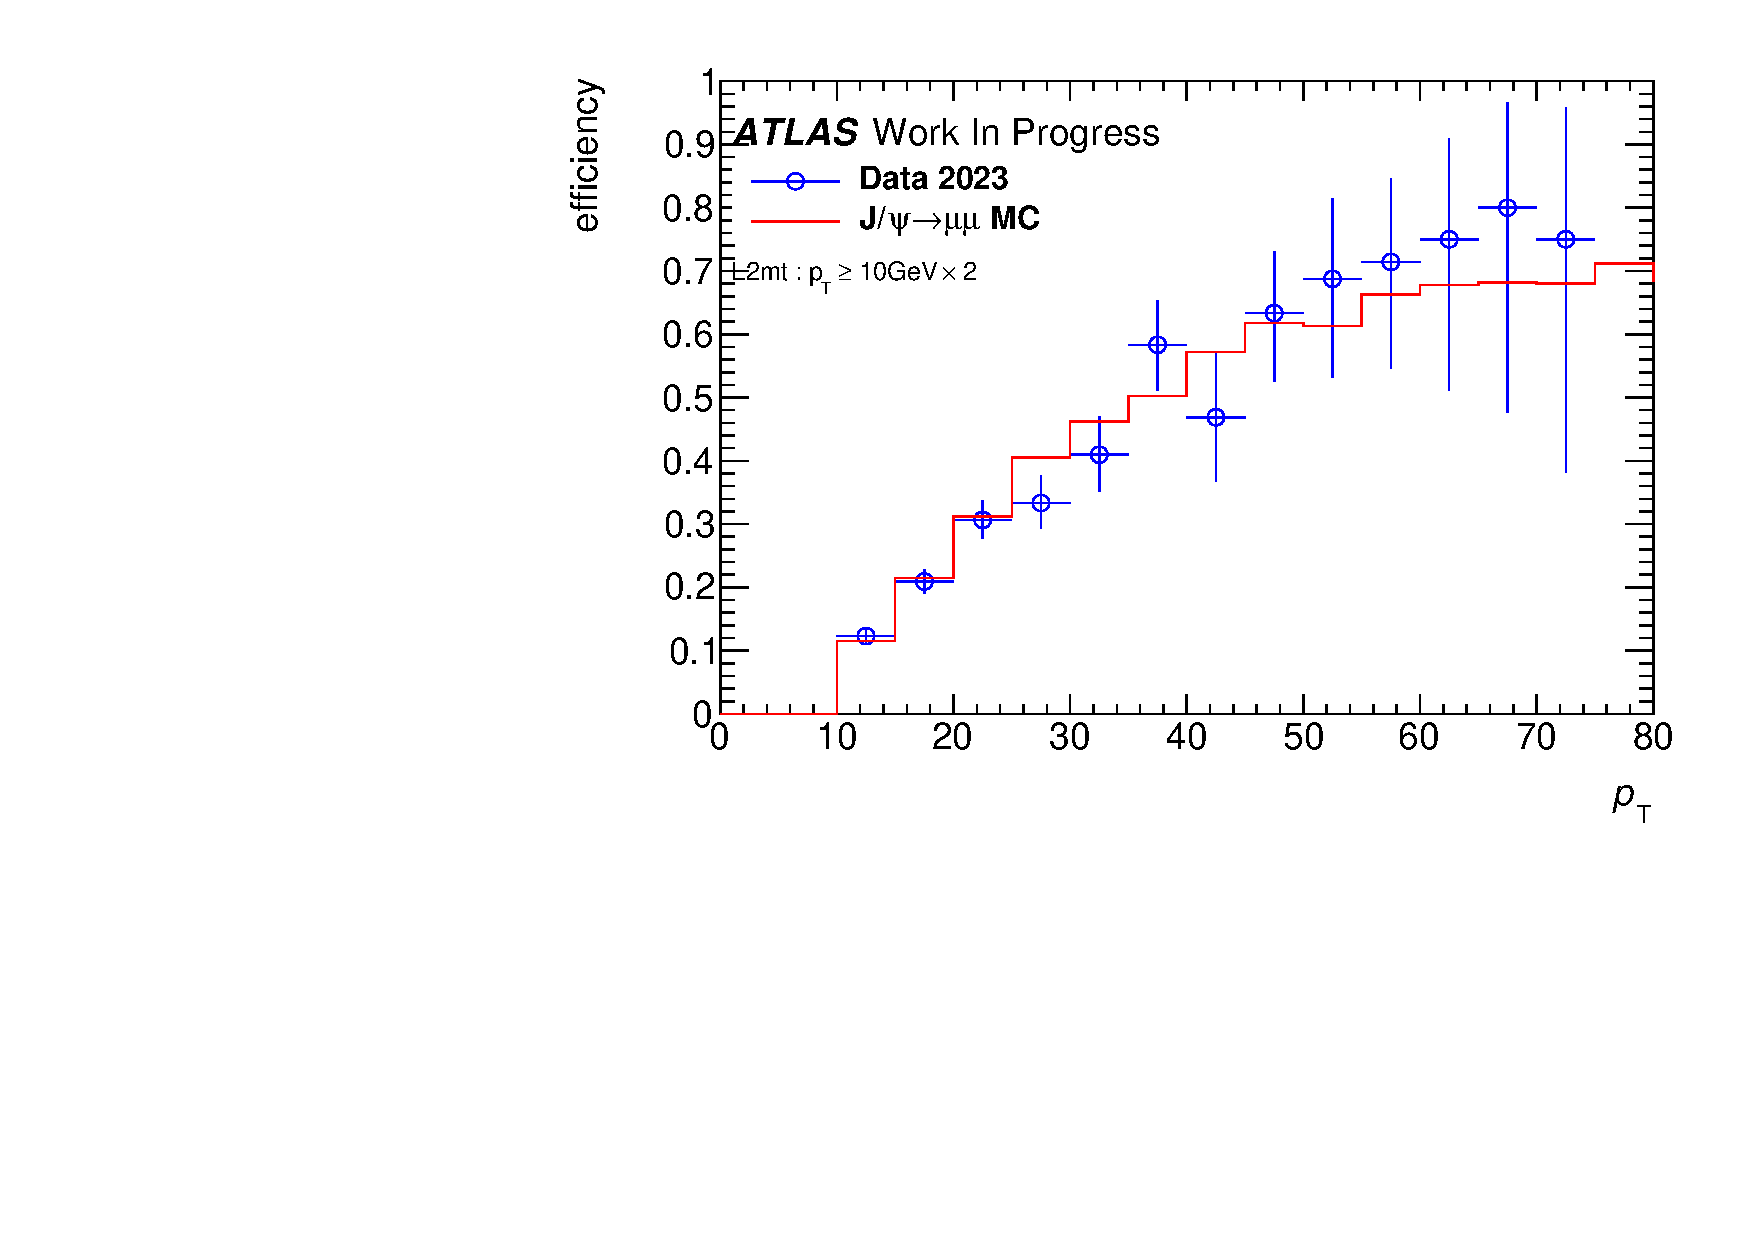
\includegraphics[clip, width=12cm]{fig/4/L2mt_eff_pt_Jpsi.pdf}
    \caption{横軸がミューオンの$\pt$でのmtSAの2つ目を見つける効率。赤線がシミュレーションでの結果、青点がデータでの結果。}
    \label{fig:L2mtPtEff}
\end{figure}

また横軸を$\pt$、2つのミューオンの不変質量である$\mathrm{M}_{\mu\mu}$の場合のトリガー効率をそれぞれ図~\ref{fig:L2mtPtEff}、図~\ref{fig:L2mtMassEff}に示す。
図~\ref{fig:L2mtMassEff}のデータの分布は$\mathrm{M}_{\mu\mu}$に対して$J/\psi$の質量の制限をかけていない。
実データでは$\pt$が$\SI{60}{\GeV}$以上のミューオンは少ないので統計誤差が大きくなっている。
また図~\ref{fig:L2mtPtEff}の$\mathrm{M}_{\mu\mu}<\SI{3}{\GeV}$の領域でシミュレーションとデータでずれているが、これはシミュレーションに用いたサンプルが$J/\psi\rightarrow\mu\mu$サンプルなので$\mathrm{M}_{\mu\mu}$が$\SI{3}{\GeV}$よりも小さい事象がほとんどなく、シミュレーションの統計誤差が大きいからである。
上記の領域以外ではシミュレーションでデータの振る舞いを再現できている。
特に、このアルゴリズムの効率が依存すると考えられる2つのミューオン同士のミューオン検出器での距離である$\Delta R_{\mu\mu~\mathrm{at~Muon~Spectrometer}}$でその分布を再現できている。
図~\ref{fig:3-13}と合わせると、2ミューオンの効率を$\Delta R_{\mu\mu~\mathrm{at~Muon~Spectrometer}}$のほぼ全領域で向上できた。

図~\ref{fig:L2mtMassEff}より2ミューオンの不変質量が$J/\psi$より小さい領域でトリガー効率が高いこと、図~\ref{fig:L2mtPtEff}より$\pt$が高くなるにつれてトリガー効率が上昇していることがわかる。
これは近接2ミューオントリガーは$J/\psi$よりも質量が小さい事象あるいはより高い$\pt$を持つ事象を対象としたトリガーなので、想定通りの結果である。